%\documentclass[a4paper,pagesize,10pt,bibtotoc,pointlessnumbers,
%normalheadings,DIV=9]{scrbook}
\documentclass[a4paper,twoside, svgnames]{article}
% twoside, openright
%\KOMAoptions{DIV=last}

%\usepackage{trajan}
 
%\usepackage[ngerman]{babel}
%\usepackage[utf8]{inputenc}
\usepackage[T1]{fontenc}
\usepackage{afterpage}

\newcommand\blankpage{%
    \null
    \thispagestyle{empty}%
    \addtocounter{page}{0}%
    \newpage}

\usepackage{pgffor, ifthen}
\newcommand{\notes}[3][\empty]{%
    \noindent Bilješke\vspace{10pt}\\
    \foreach \n in {1,...,#2}{%
        \ifthenelse{\equal{#1}{\empty}}
            {\rule{#3}{0.5pt}\\}
            {\rule{#3}{0.5pt}\vspace{#1}\\}
        }
}

%=========================================
%   INCLUDE CUSTOM PAKETA
%=========================================
\usepackage{fontspec}
 
% JohnSansTextPro
\setromanfont[
Path=fonts/,
BoldFont=JohnSansTextBold.ttf,
ItalicFont=JohnSansTextItalic.ttf,
BoldItalicFont=JohnSansTextBoldItalic.ttf
]{JohnSansText.ttf}

% JohnSansMediumPro
\setsansfont[
Path=fonts/,
BoldFont=JohnSansMediumProBold.ttf,
ItalicFont=JohnSansMediumProItalic.ttf,
BoldItalicFont=JohnSansMediumProBoldItalic.ttf
]{JohnSansMediumPro.ttf}

% JohnSansWhitePro
\setmonofont[Scale=1,
Path=fonts/,
BoldFont=JohnSansWhiteBold.ttf,
ItalicFont=JohnSansWhiteItalic.ttf,
BoldItalicFont=JohnSansWhiteBoldItalic.ttf
]{JohnSansWhite.ttf}

\usepackage{setspace}
\usepackage{pdfpages}
\usepackage{xcolor}
\usepackage{fancyhdr}
\pagestyle{fancy}

\fancyhead{}
\fancyfoot{}
\fancyfoot[RO,LE]{\rmfamily\thepage}
\renewcommand{\headrulewidth}{0pt} \renewcommand{\footrulewidth}{0pt} 
\includepdfset{pagecommand=\thispagestyle{fancy}}
%\setlength{\footrulewidth}{-10mm}

%parametri za brojeve str BEZ geometry paketa
%\setlength{\footskip}{-26.5mm}
%\fancyfootoffset[R]{15.5mm}
%\fancyfootoffset[L]{15.5mm}

%parametri za brojeve str SA geometry paketa
%\setlength{\footskip}{-38mm}
\fancyfootoffset[R]{4mm}
\fancyfootoffset[L]{4mm}

%\usepackage{hyperref}
%\hypersetup{
%    colorlinks,
%    citecolor=black,
%    filecolor=black,
%    linkcolor=black,
%    urlcolor=black,
%    linktoc=all
%%}
\usepackage[colorlinks=false,pdfborder={0 0 0},pdfpagelabels]{hyperref}
%\hypersetup{linktocpage}
%\usepackage[all]{hypcap}

%\usepackage{titlesec}
%\usepackage{geometry}
%\usepackage[hmarginratio=1:1]{geometry}
\usepackage[footskip=34pt, hmarginratio=1:1, left=20mm, bottom=24mm, top=31.4mm]{geometry}
\usepackage{graphicx}

%crop za stampu
%\usepackage[
%  % set width and height to a4 width and height + 6mm
%  width=21.6truecm, height=30.3truecm,
%  % use any combination of these options to add different cut markings
%  cam, axes, frame, cross,
%  % set the type of TeX renderer you use
%  pdftex,
%  % center the contents
%  center
%]{crop}

%\multicolumn paket za tekst
\usepackage{multicol}
\usepackage{wrapfig}
\setlength{\columnsep}{1cm}
\usepackage{ragged2e}
\usepackage{caption}


%za mijenjanje TOCa
\usepackage[]{tocloft}

%za namjestanje margina po stranici
\usepackage{changepage}

%=========================================
%   CUSTOM VARIABLES
%=========================================
\newcommand{\doccolor}{\color{farmfest}}
\newcommand{\twodigitspacing}{5pt}
\newcommand{\onedigitspacing}{11.8pt}
\newcommand{\impresspac}{7pt}
\newcommand{\rednifont}{\sffamily}
\definecolor{farmfest}{RGB}{153,85,255}
%\definecolor{farmfest}{RGB}{56,182,255}
%\definecolor{anker}{RGB}{250,162,31}

%=========================================
%   TITLE PAGE CUSTOMIZATION
%=========================================
\newcommand*{\titleTH}{\begingroup
\vspace*{5cm}
\begin{center}
{{\fontsize{63.3}{70}\selectfont
\textsf{{PJESMARICA}}}}\\
\vspace*{0.3cm}
{{\fontsize{50}{60}\selectfont
\textsf{\textcolor{farmfest}{FARMFEST 2026}}}}
\vfill % Whitespace between the title block and the publisher
\includegraphics[width=0.2\linewidth]{images/ff_22}\\
%\vspace*{0.5cm}
%{Pušćine, 2022.}\par % Publisher and logo
%\vspace*{3\baselineskip} % Whitespace at the bottom of the page
\end{center}
\endgroup}

%#################################################################################
%   BEGINING OF DOCUMENT
%#################################################################################
%=========================================
%   TITLE PAGE
%=========================================
\begin{document}
%Cover page
\newpage
\pagenumbering{gobble} 
\includepdf[pages={1},noautoscale]{images/ff2026_korice_prednja_eb.pdf}

\newpage
\pagenumbering{gobble}
\vspace*{10.7cm}
%\begin{center}
%    Inner side of front cover page. Remove!
%\end{center}
%\begin{center}
%    \textit{Unutarnja strana korica.}
%\end{center}

%Title page
\newpage
\pagenumbering{gobble} 
\thispagestyle {empty}
%\titleTH

\includepdf[pages={1},noautoscale]{images/pjesmarica_crni_logo.pdf}
%=========================================
%   IMPRESSUM
%=========================================
\newpage
%\centering
\thispagestyle {empty}
\pagenumbering{arabic}
\setcounter{page}{2}
\begin{center}
\vspace*{\fill}
\begin{onehalfspacing}
%\textbf{\textsf{Impressum}}\\
%\vspace{10pt}
\textbf{Naslov:} Farmfest pjesmarica 2026\\
\vspace{\impresspac}
%\textbf{Izdanje:} Srpanj 2026.\\
%\vspace{\impresspac}
\textbf{Izdavač:} "Riječi Iskrene" Dravska 8, 40305 Pušćine, Hrvatska\\
\vspace{\impresspac}
\textbf{Kontakt:} www.farmfest.eu\\
\vspace{\impresspac}
\textbf{Zapis nota:} Stjepan i Benjamin Horvat | Lilypond 2.24.4 (http://lilypond.org)\\
\vspace{\impresspac}
\textbf{Naslovnica i poleđina:} Ruben Horvat\\
\vspace{\impresspac}
\textbf{Logotip:} Mario Jekić\\
\vspace{\impresspac}
\textbf{Priprema:} Benjamin Horvat | LaTeX (http://latex-project.org)\\
\vspace{\impresspac}
\textbf{Prijevod:} Filip Horvat, Daniel Kreko, Andrea Horvat\\
\vspace{\impresspac}
\textbf{Lektura:} Nenad Pijanić, Anja Kovačević\\
\vspace{\impresspac}
\textbf{Korektura:} Benjamin Horvat\\
\vspace{\impresspac}
\textbf{Fotografije:} Filip Horvat\\
\vspace{\impresspac}
\textbf{Tisak:} Stefil d.o.o.\\
\vspace{\impresspac}
%Tekst i glazba: Frank Bosch\\
%\vspace{\impresspac}
\textbf{Licenca:} Creative Commons—Attribution-ShareAlike 4.0\\
\vspace{\impresspac}
%“Farmfest” Dravska 8, 40000 Čakovec, Hrvatska\\
\vspace{\impresspac}
\vspace{\impresspac}
\vspace{\impresspac}

\end{onehalfspacing}
\end{center}

%=========================================
%   TOC
%=========================================
\newpage
\begin{adjustwidth*}{2cm}{2cm}
\renewcommand{\cftsecfont}{\rmfamily}
\renewcommand{\cftsecpagefont}{\sffamily}
\renewcommand{\cfttoctitlefont}{\rmfamily\fontsize{50}{60}\selectfont}
\renewcommand{\contentsname}{
    {\rmfamily\hfill\doccolor Kazalo \hfill}
    
    \vspace*{0.5cm}
    
    {\Huge\hfill \textit{Farmfest 2026} \hfill}
}
\renewcommand{\cftaftertoctitle}{\vspace*{2cm}}
\vspace*{1cm}
{\large{
\addtocontents{toc}{\protect\enlargethispage{-25mm}}
%\clearpage
\tableofcontents}}
\thispagestyle{empty}
\end{adjustwidth*}

%\afterpage{\blankpage}

%=========================================
%   PJESME
%=========================================
%pjesma 1
\addtocontents{toc}{\protect\thispagestyle{empty}}
\newpage
\phantomsection
\begin{minipage}[b]{0.5\linewidth}
\addcontentsline{toc}{section}{\texorpdfstring{{\rednifont\doccolor1.}\hspace{\onedigitspacing}}{}BEZ LJUBAVI}
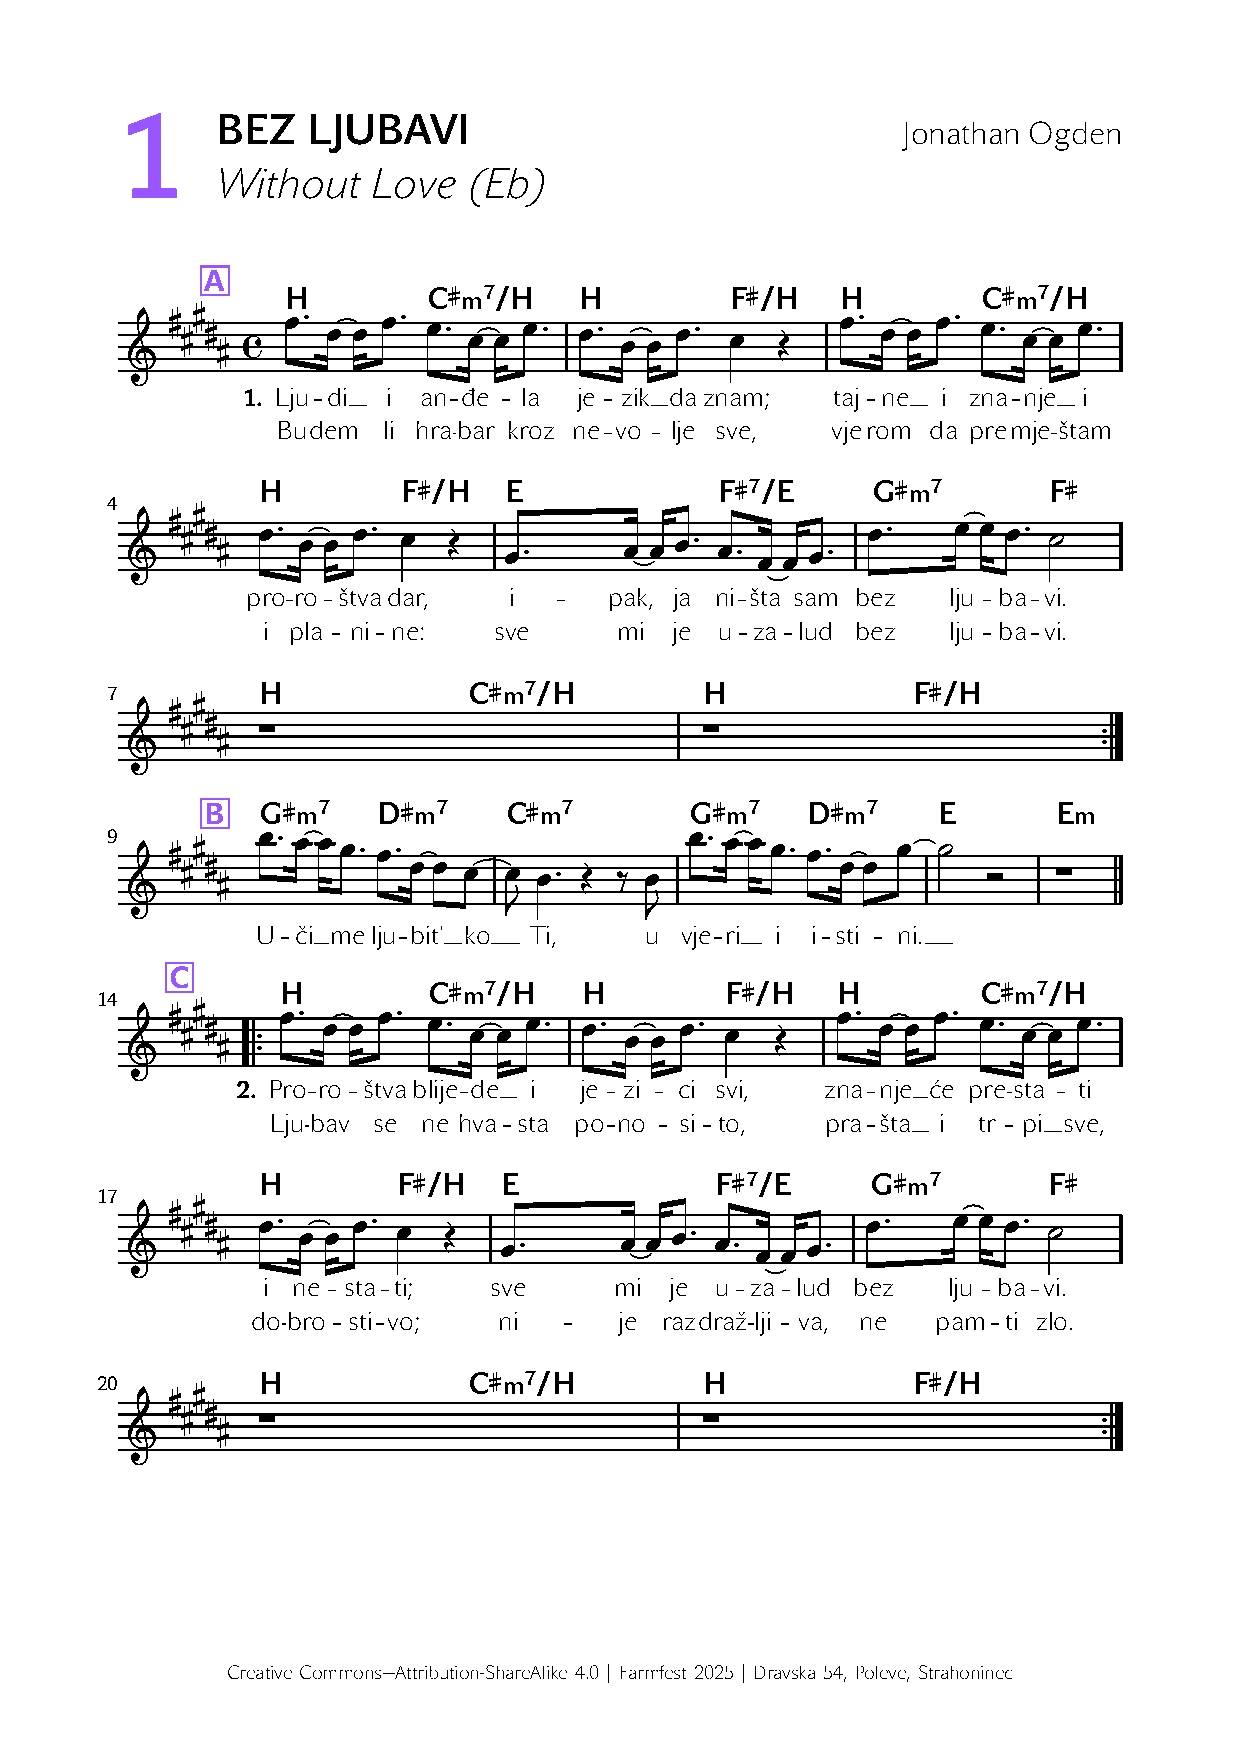
\includepdf[pages={1},noautoscale]{../lilypond/bin_eb/bez_ljubavi.pdf}
\end{minipage}
\newpage
\includepdf[pages={2},noautoscale,
    picturecommand={\setlength\unitlength{1cm}%
         \put(2,3.4){\includegraphics[width=\linewidth]{images/2.jpg}}}]%
   {../lilypond/bin_eb/bez_ljubavi.pdf}

%pjesma 2
\newpage
\phantomsection
\begin{minipage}[b]{0.5\linewidth}
\addcontentsline{toc}{section}{\texorpdfstring{{\rednifont\doccolor2.}\hspace{\onedigitspacing}}{}BOG JE MOJA SNAGA}
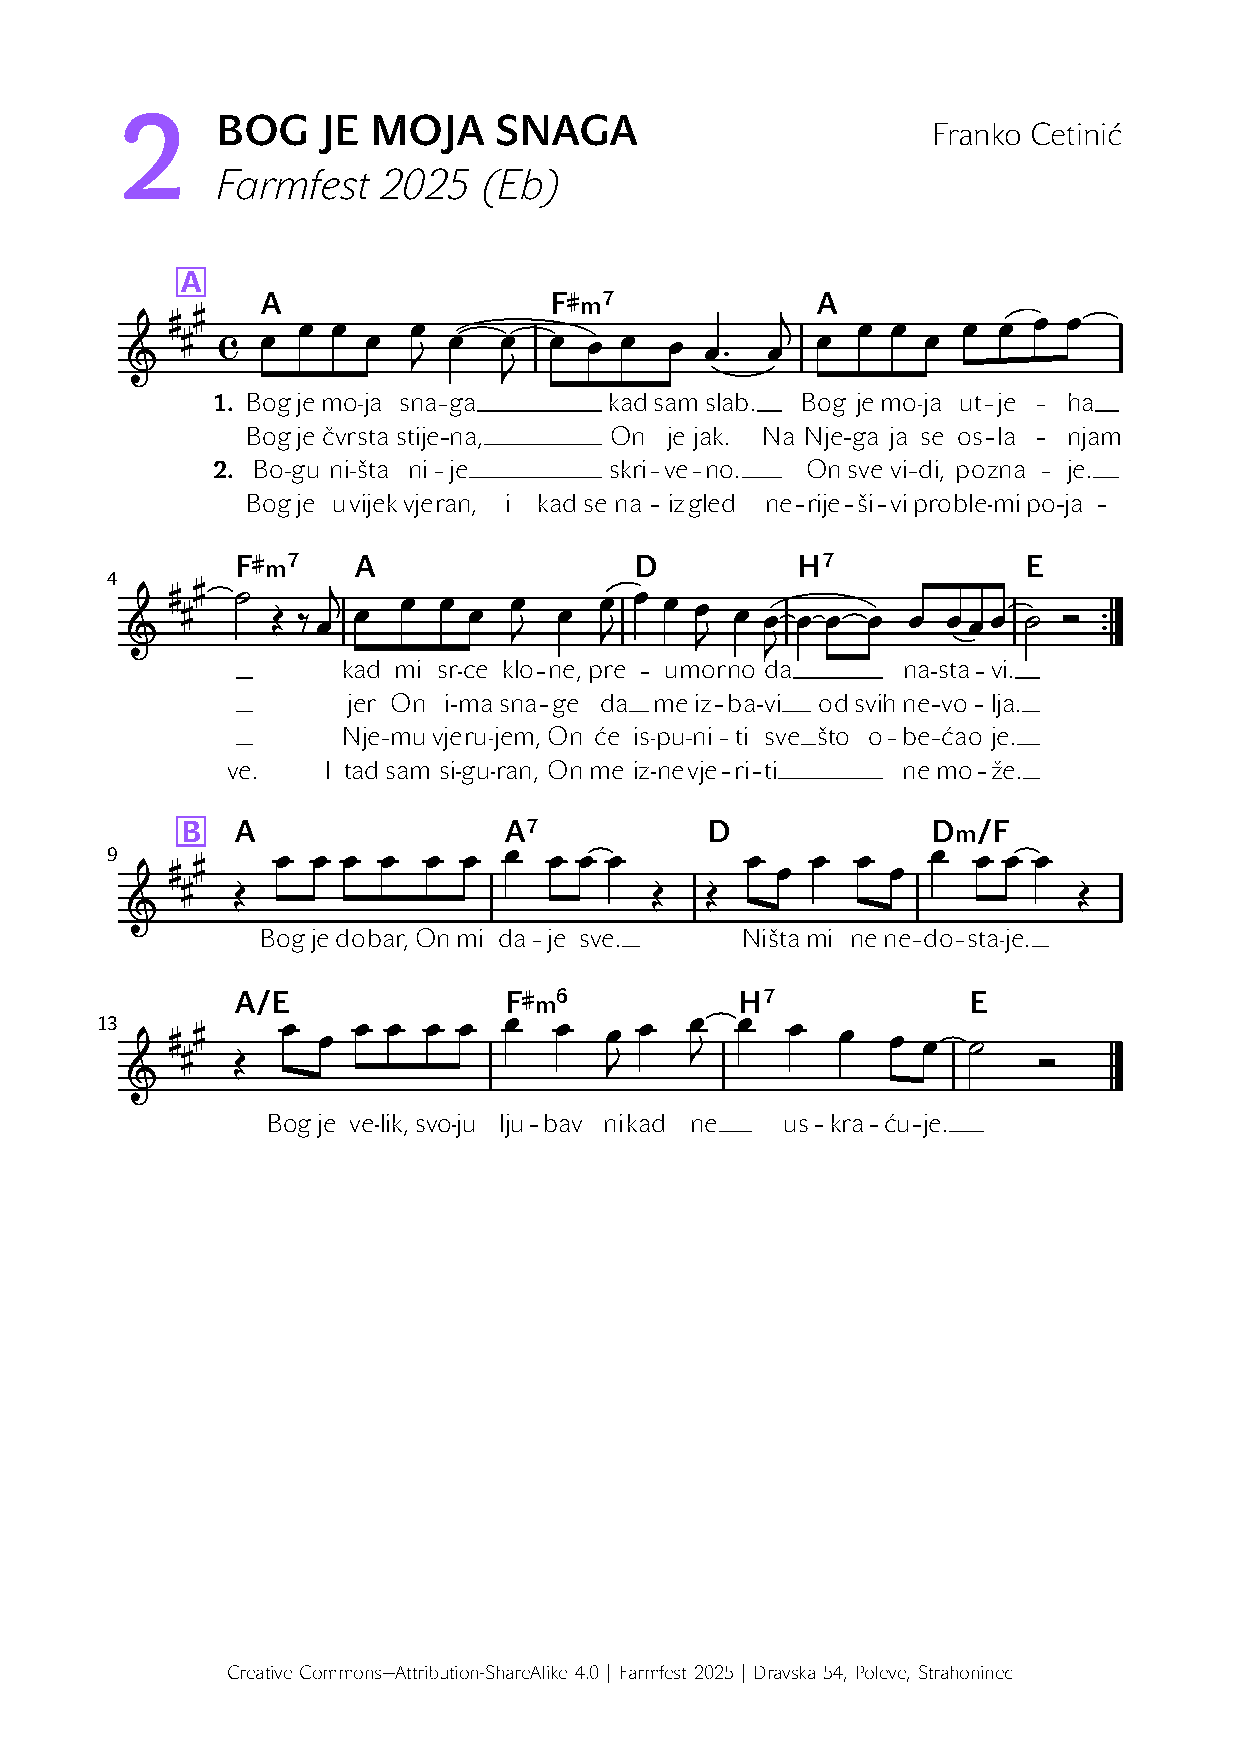
\includepdf[pages={1},noautoscale]{../lilypond/bin_eb/bog_je_moja_snaga.pdf}
\end{minipage}

%pjesma 3
\newpage
\phantomsection
\begin{minipage}[b]{0.5\linewidth}
\addcontentsline{toc}{section}{\texorpdfstring{{\rednifont\doccolor3.}\hspace{\onedigitspacing}}{}IME ISUS}
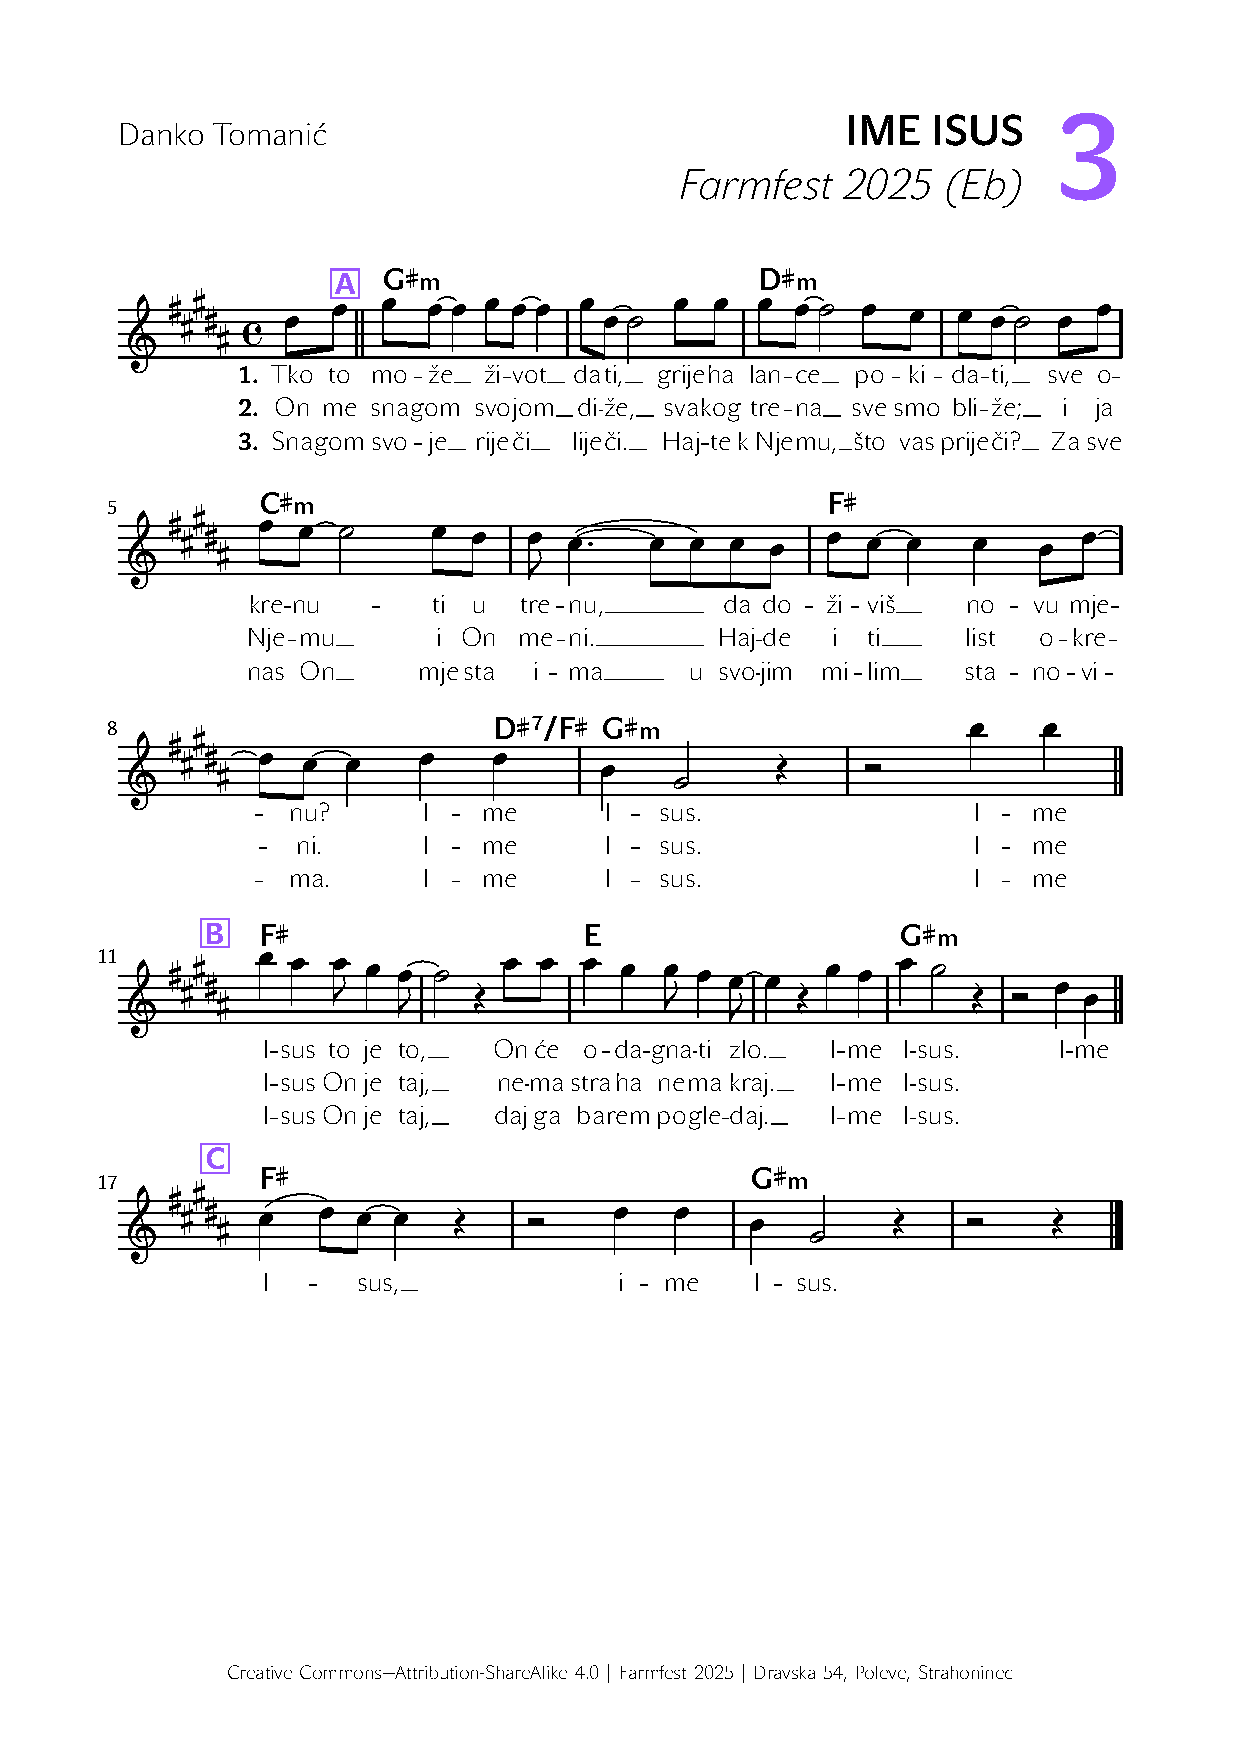
\includepdf[pages={1},noautoscale]{../lilypond/bin_eb/ime_isus.pdf}
\end{minipage}

%pjesma 4
\newpage
\phantomsection
\begin{minipage}[b]{0.5\linewidth}
\addcontentsline{toc}{section}{\texorpdfstring{{\rednifont\doccolor4.}\hspace{\onedigitspacing}}{}ISUS NAZAREĆANIN}
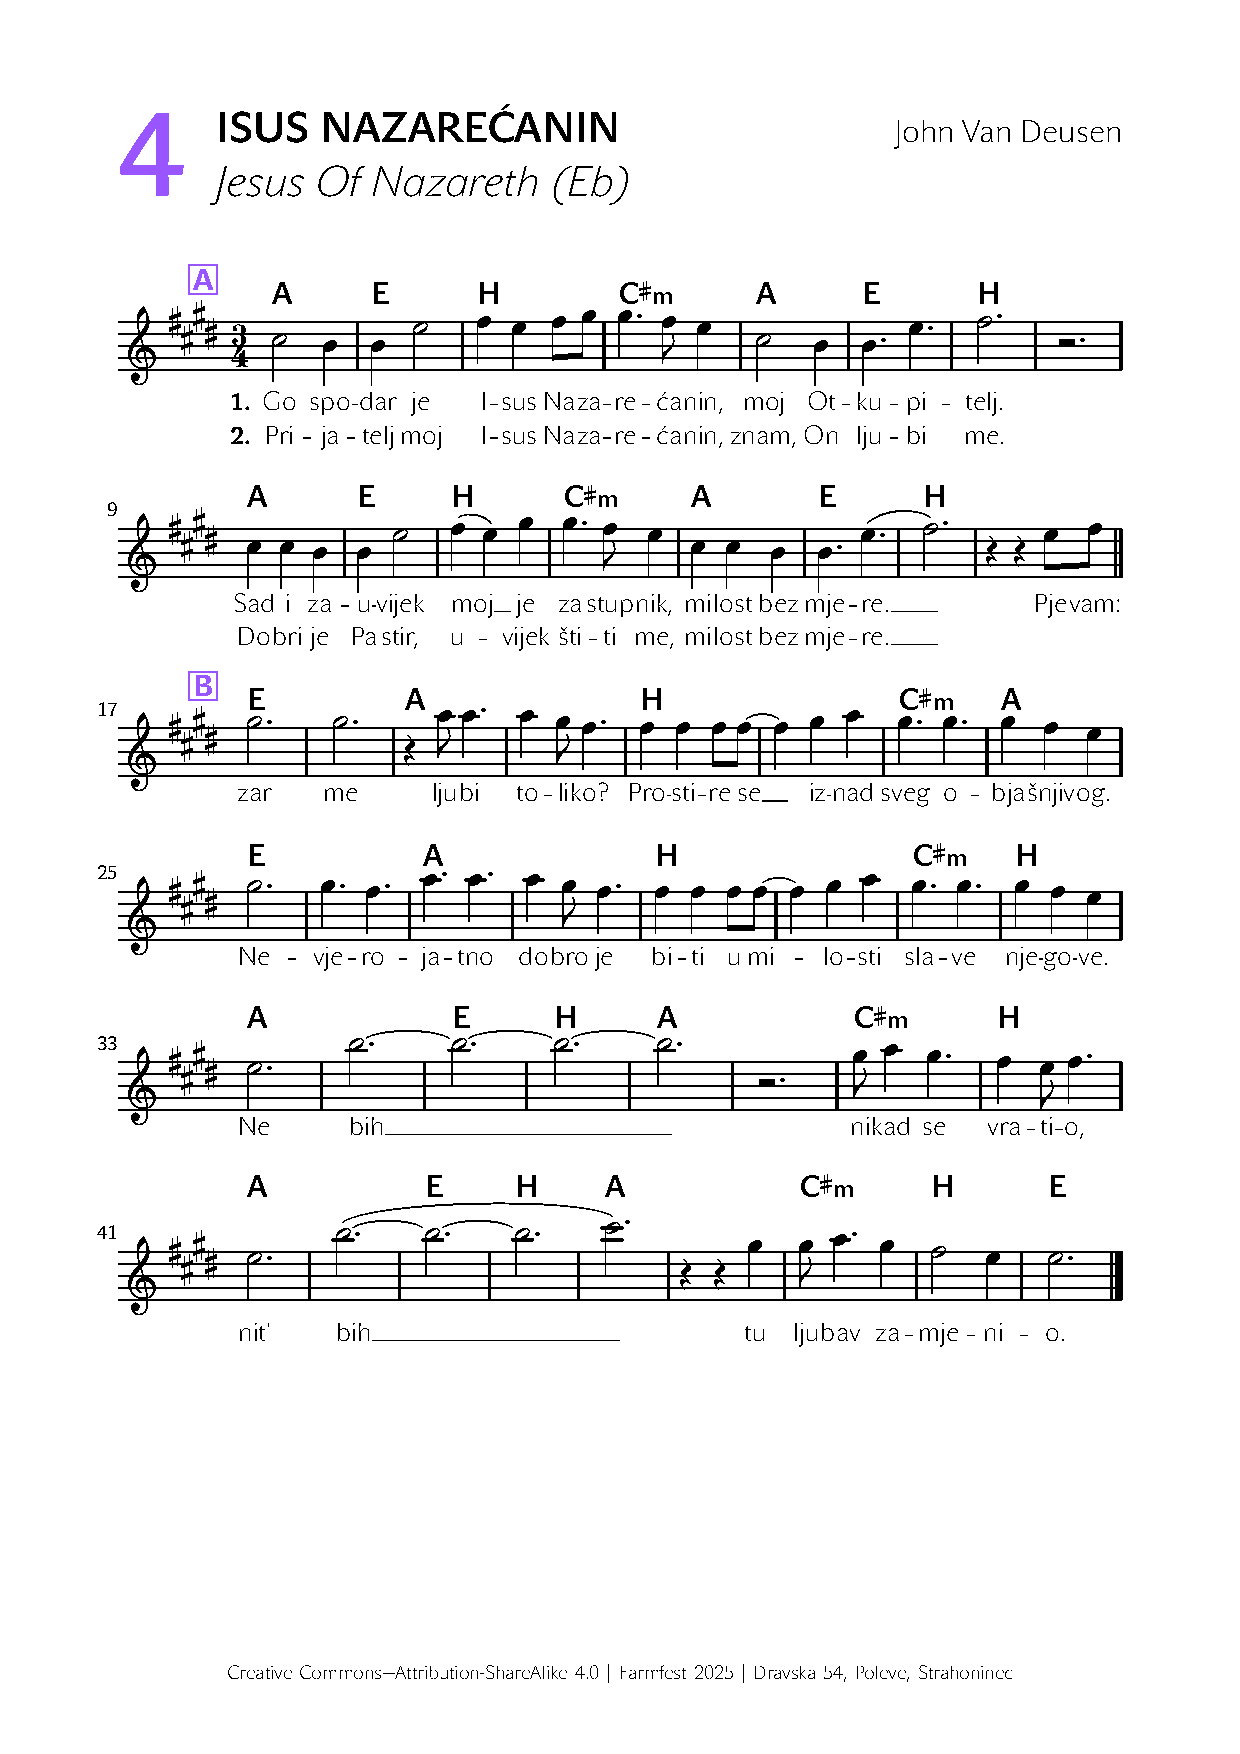
\includepdf[pages={1},noautoscale]{../lilypond/bin_eb/isus_nazarecanin.pdf}
\end{minipage}

%slika
\newpage
%\vspace*{4cm}

\begin{center}
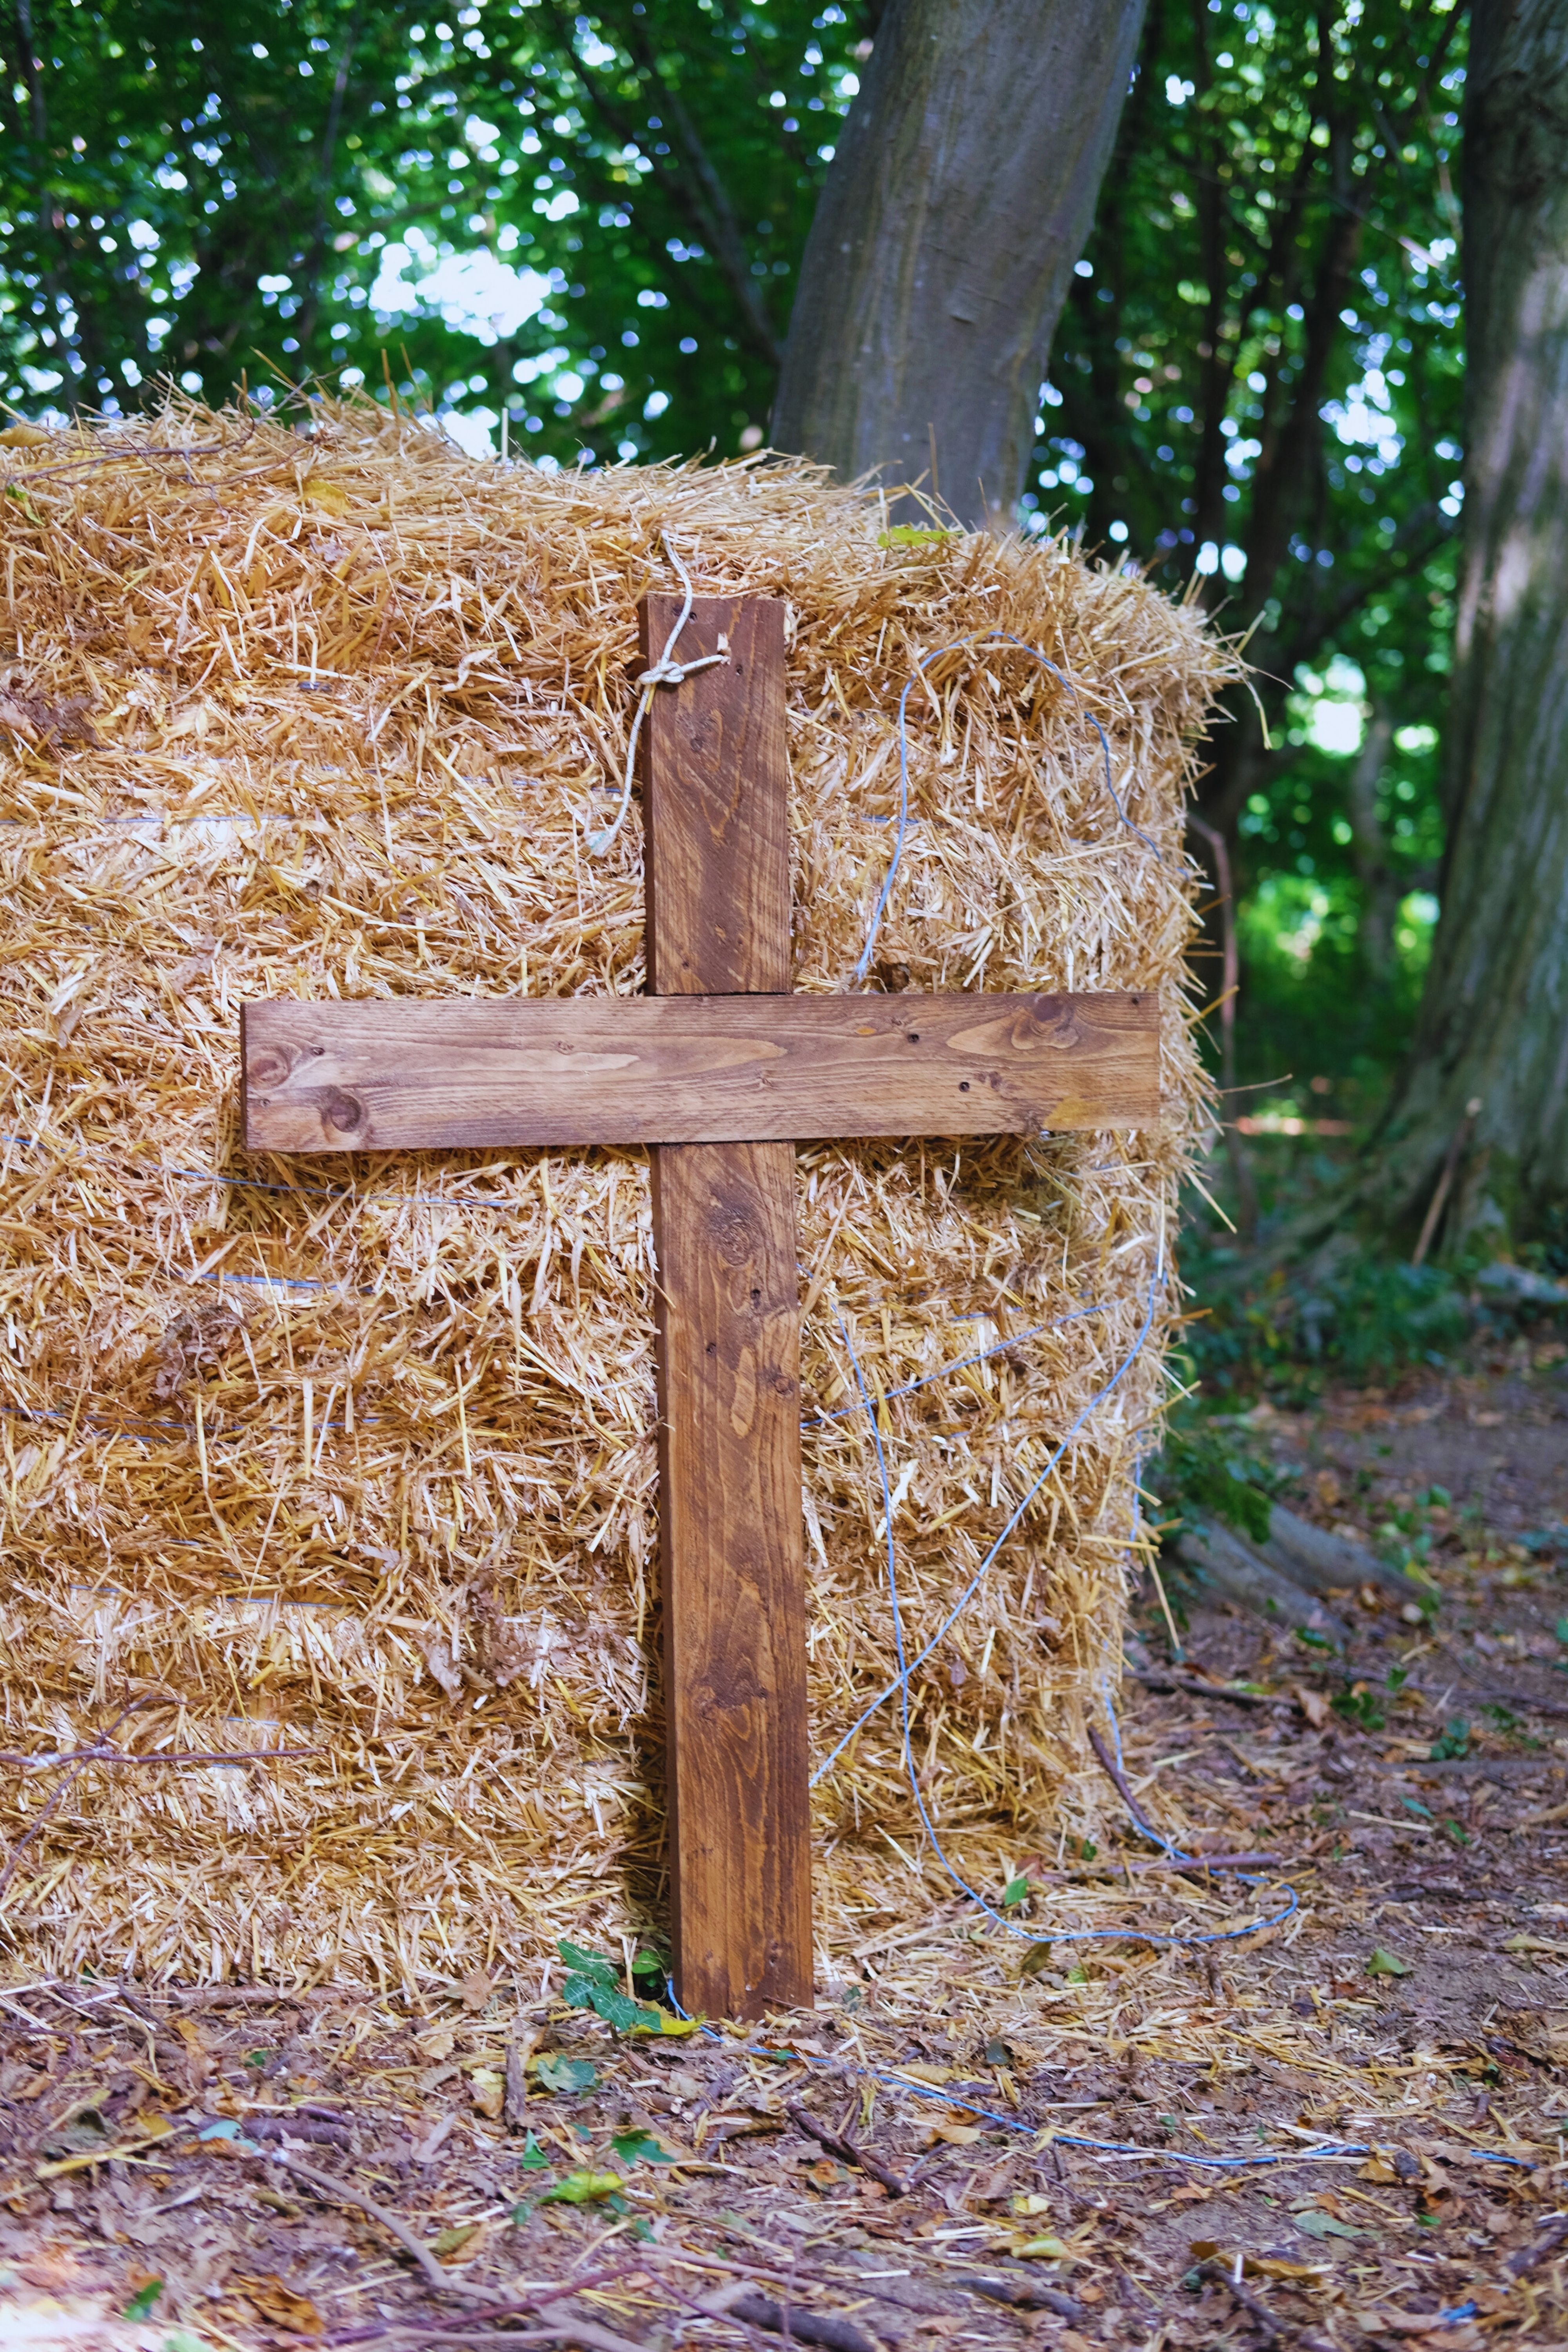
\includegraphics[width=400pt]{images/34.jpg}
\end{center}

\vspace*{1mm}
\begin{center}

	\Large{\parbox{\linewidth}{
		\begin{center}
		{\Large
		\texttt{
			\textit{"Ja sam put, istina i život \textemdash{ } reče Isus.\\\textemdash Nitko ne dolazi k Ocu osim po meni."}
			}
		}
		\end{center}
		\begin{center}
		{\Large
			\texttt{{\textemdash Ivan 14,6}}
		}
		\end{center}
	}
}
\end{center}

%pjesma 5
\newpage
\phantomsection
\begin{minipage}[b]{0.5\linewidth}
\addcontentsline{toc}{section}{\texorpdfstring{{\rednifont\doccolor5.}\hspace{\onedigitspacing}}{}PASTIR MOJE DUŠE}
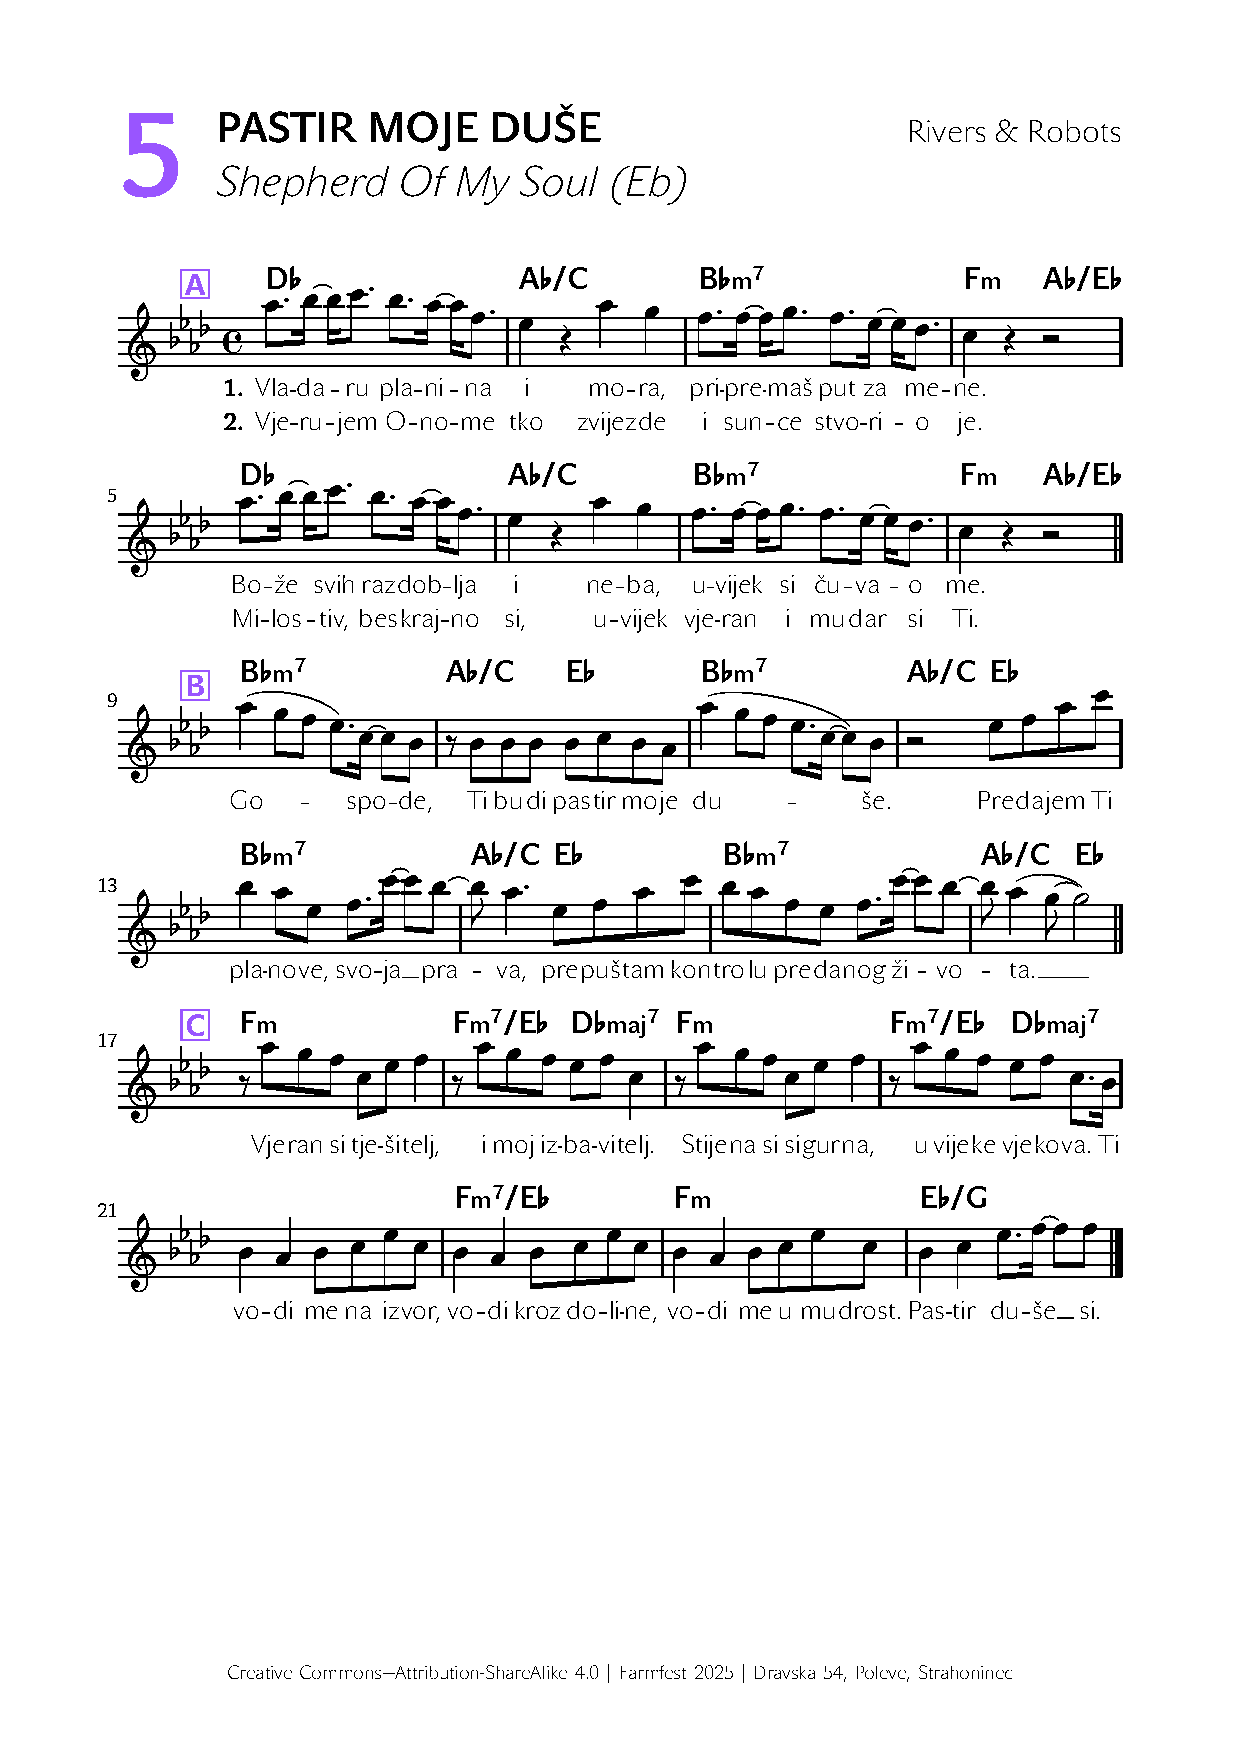
\includepdf[pages={1},noautoscale]{../lilypond/bin_eb/pastir_moje_duse.pdf}
\end{minipage}

%pjesma 6
\newpage
\phantomsection
\begin{minipage}[b]{0.5\linewidth}
\addcontentsline{toc}{section}{\texorpdfstring{{\rednifont\doccolor6.}\hspace{\onedigitspacing}}{}POZIV}
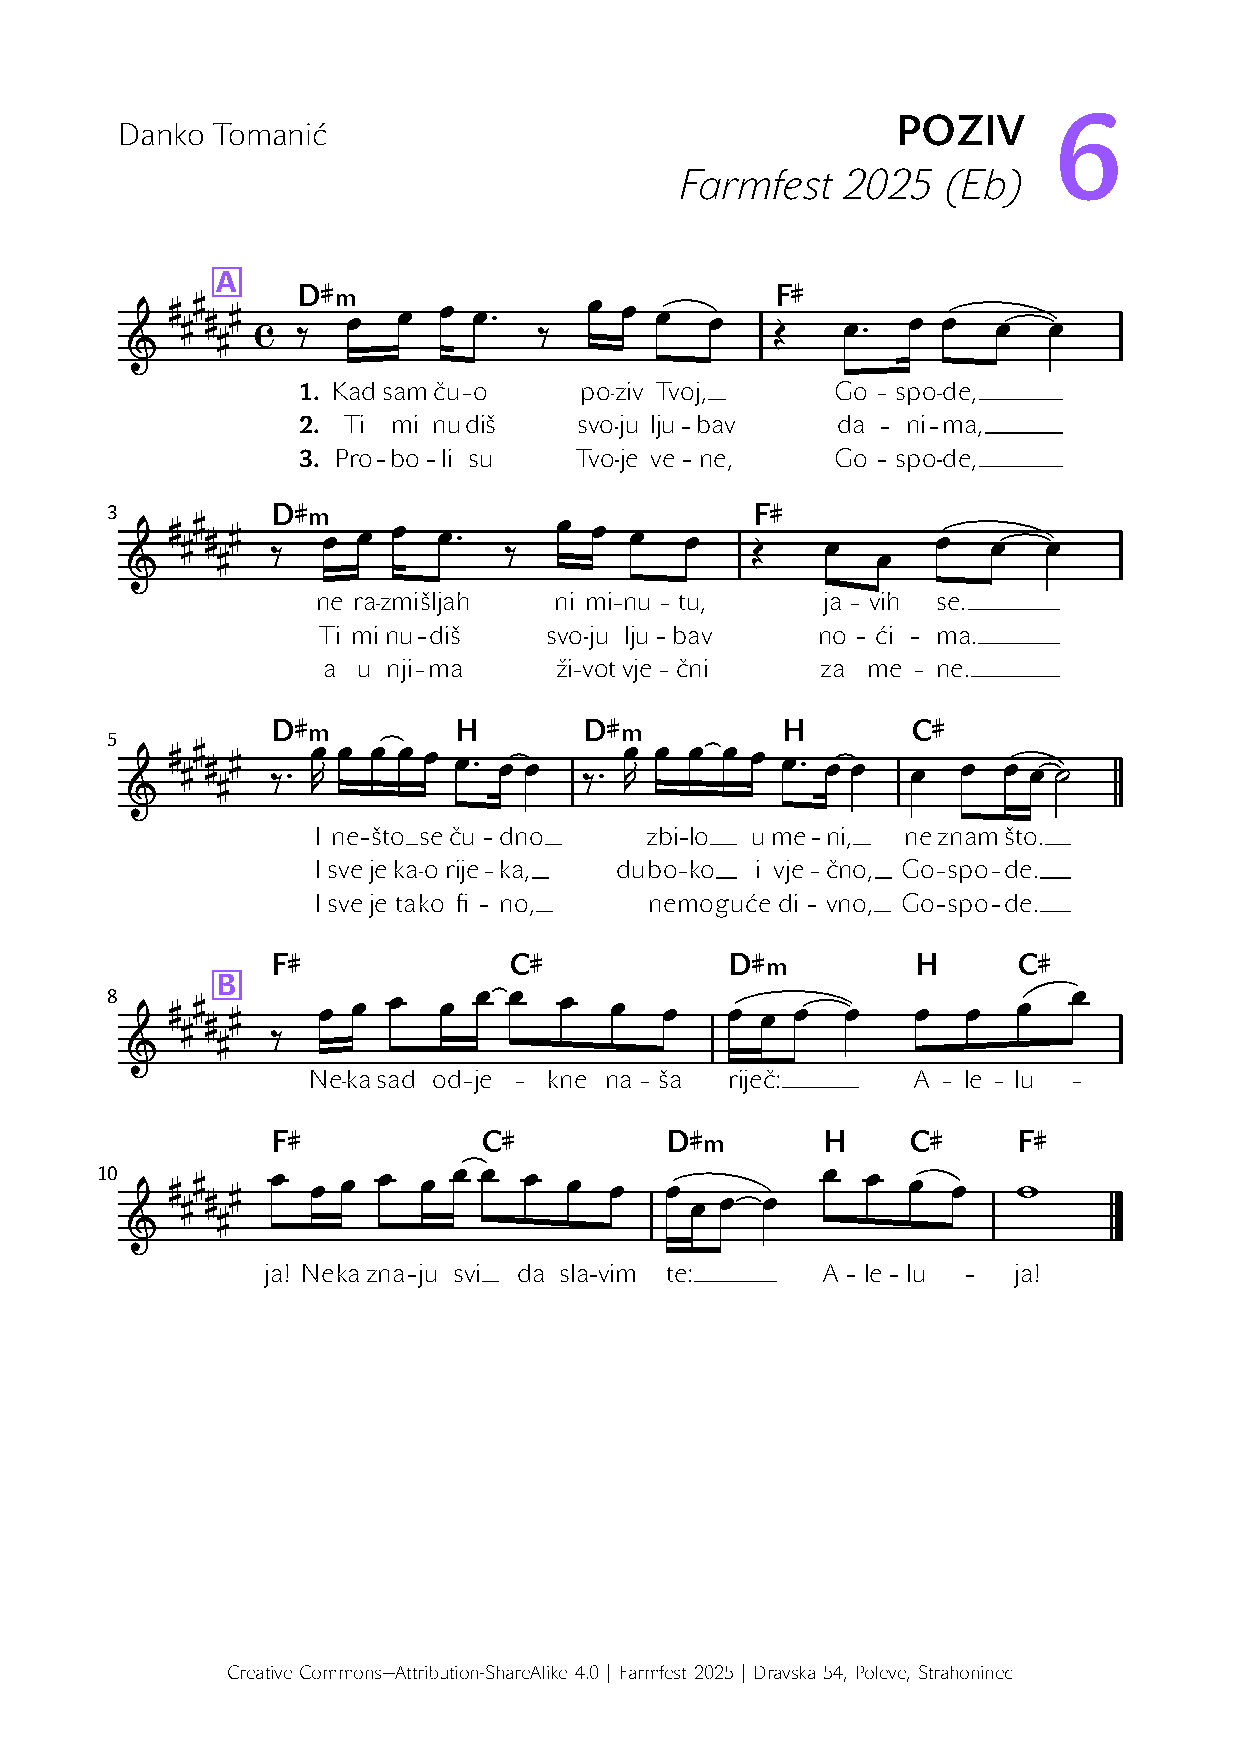
\includepdf[pages={1},noautoscale]{../lilypond/bin_eb/poziv.pdf}
\end{minipage}

%pjesma 7
\newpage
\phantomsection
\begin{minipage}[b]{0.5\linewidth}
\addcontentsline{toc}{section}{\texorpdfstring{{\rednifont\doccolor7.}\hspace{\onedigitspacing}}{}PSALAM 42}
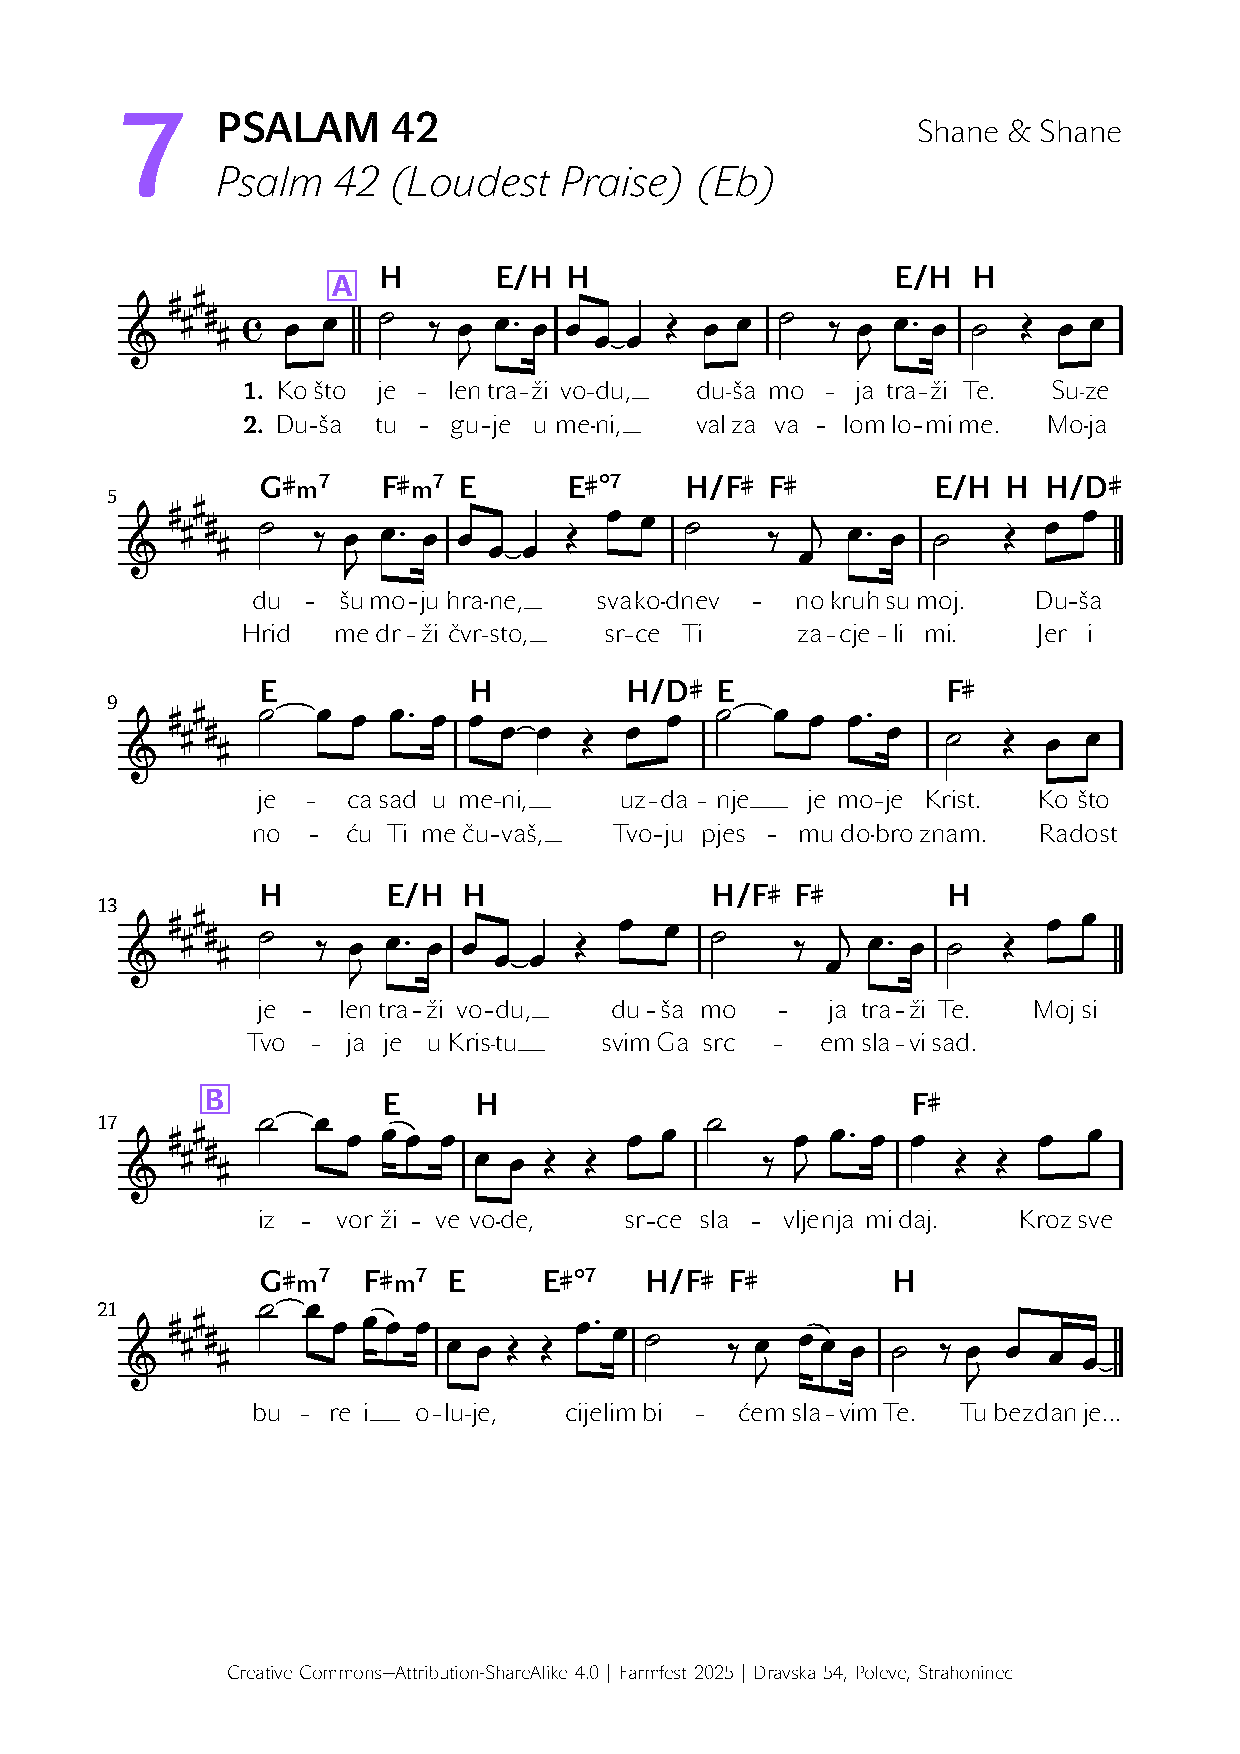
\includepdf[pages={1},noautoscale]{../lilypond/bin_eb/psalam_42.pdf}
\end{minipage}
\newpage
\includepdf[pages={2},noautoscale,
    picturecommand={\setlength\unitlength{1cm}%
         \put(2,4.5){\includegraphics[width=\linewidth]{images/4.jpg}}}]%
   {../lilypond/bin_eb/psalam_42.pdf}

%pjesma 8
\newpage
\phantomsection
\begin{minipage}[b]{0.5\linewidth}
\addcontentsline{toc}{section}{\texorpdfstring{{\rednifont\doccolor8.}\hspace{\onedigitspacing}}{}TO DADE BOG}
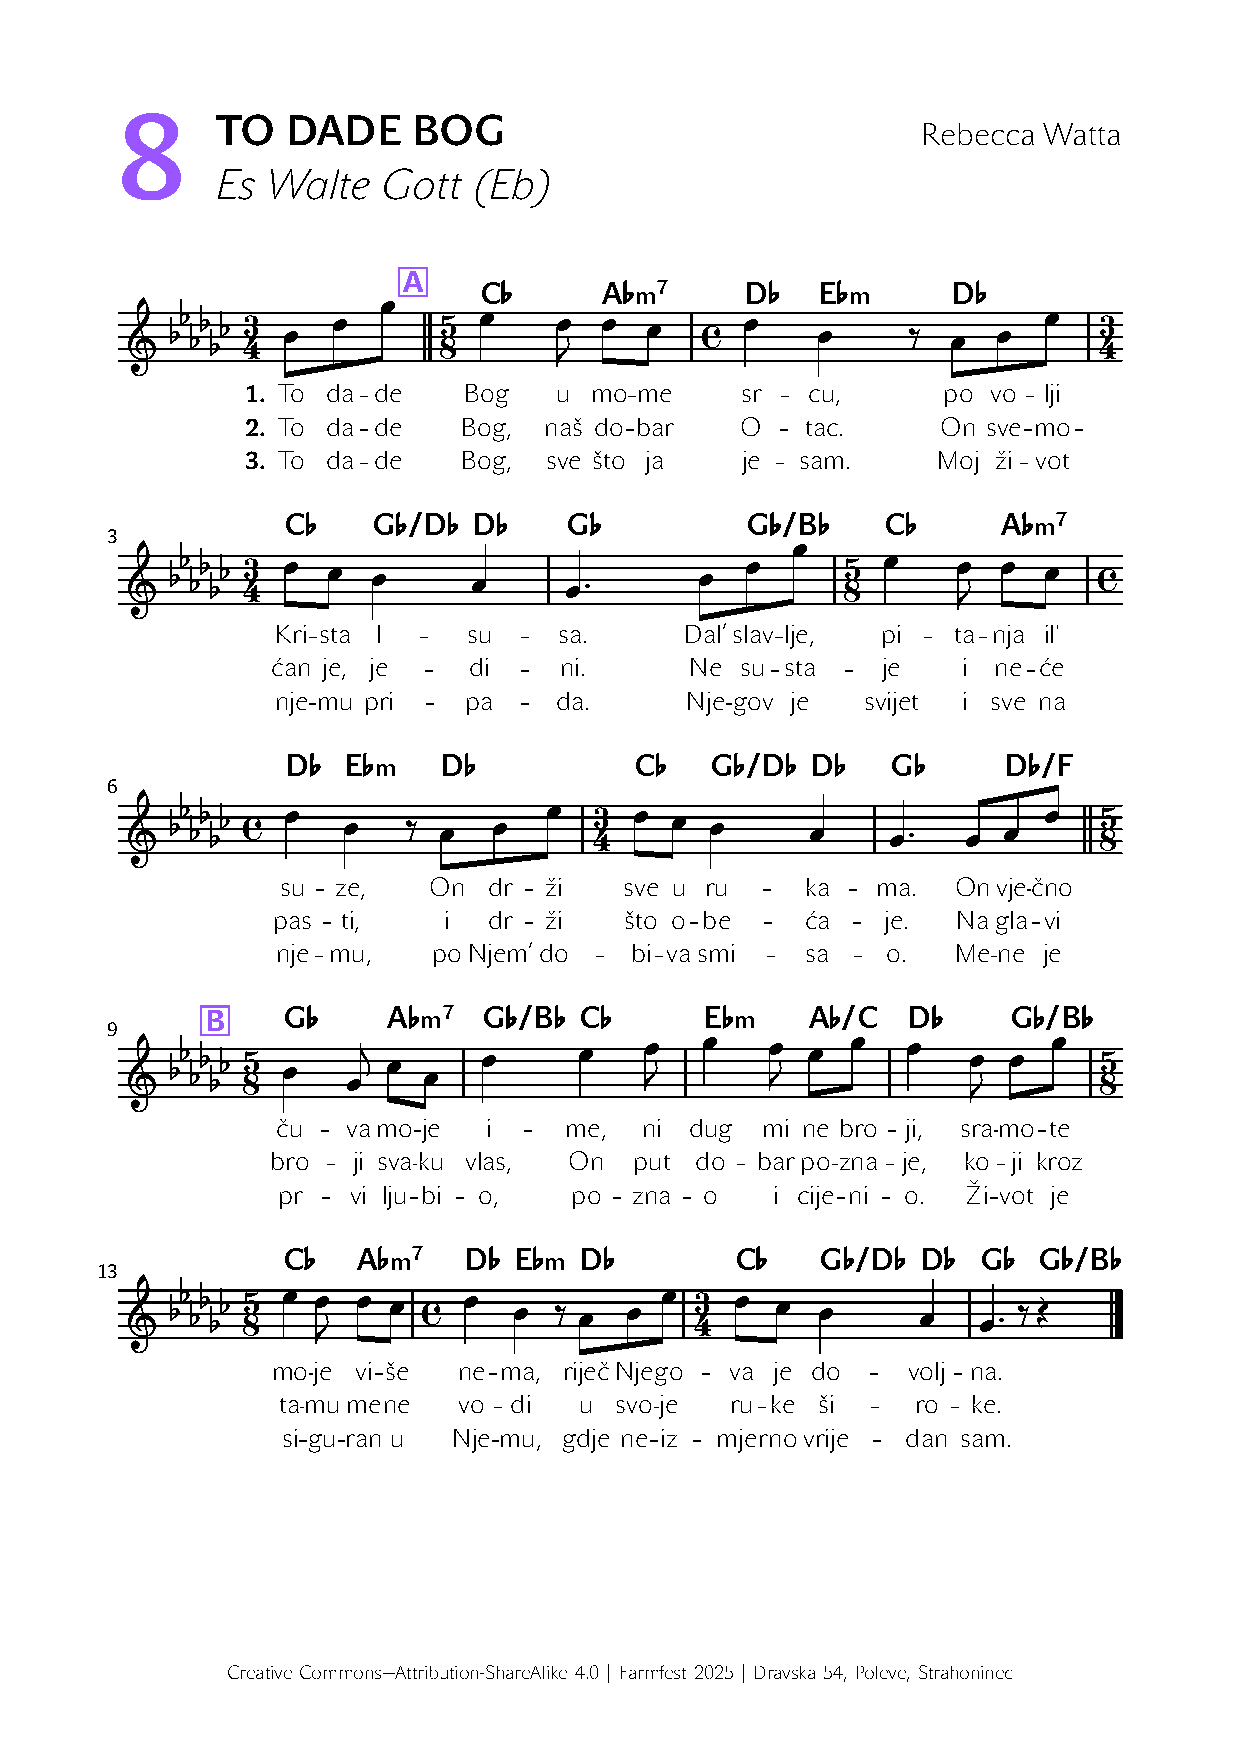
\includepdf[pages={1},noautoscale]{../lilypond/bin_eb/to_dade_bog.pdf}
\end{minipage}

%pjesma 9
\newpage
\phantomsection
\begin{minipage}[b]{0.5\linewidth}
\addcontentsline{toc}{section}{\texorpdfstring{{\rednifont\doccolor9.}\hspace{\onedigitspacing}}{}TVOJE NEBO}
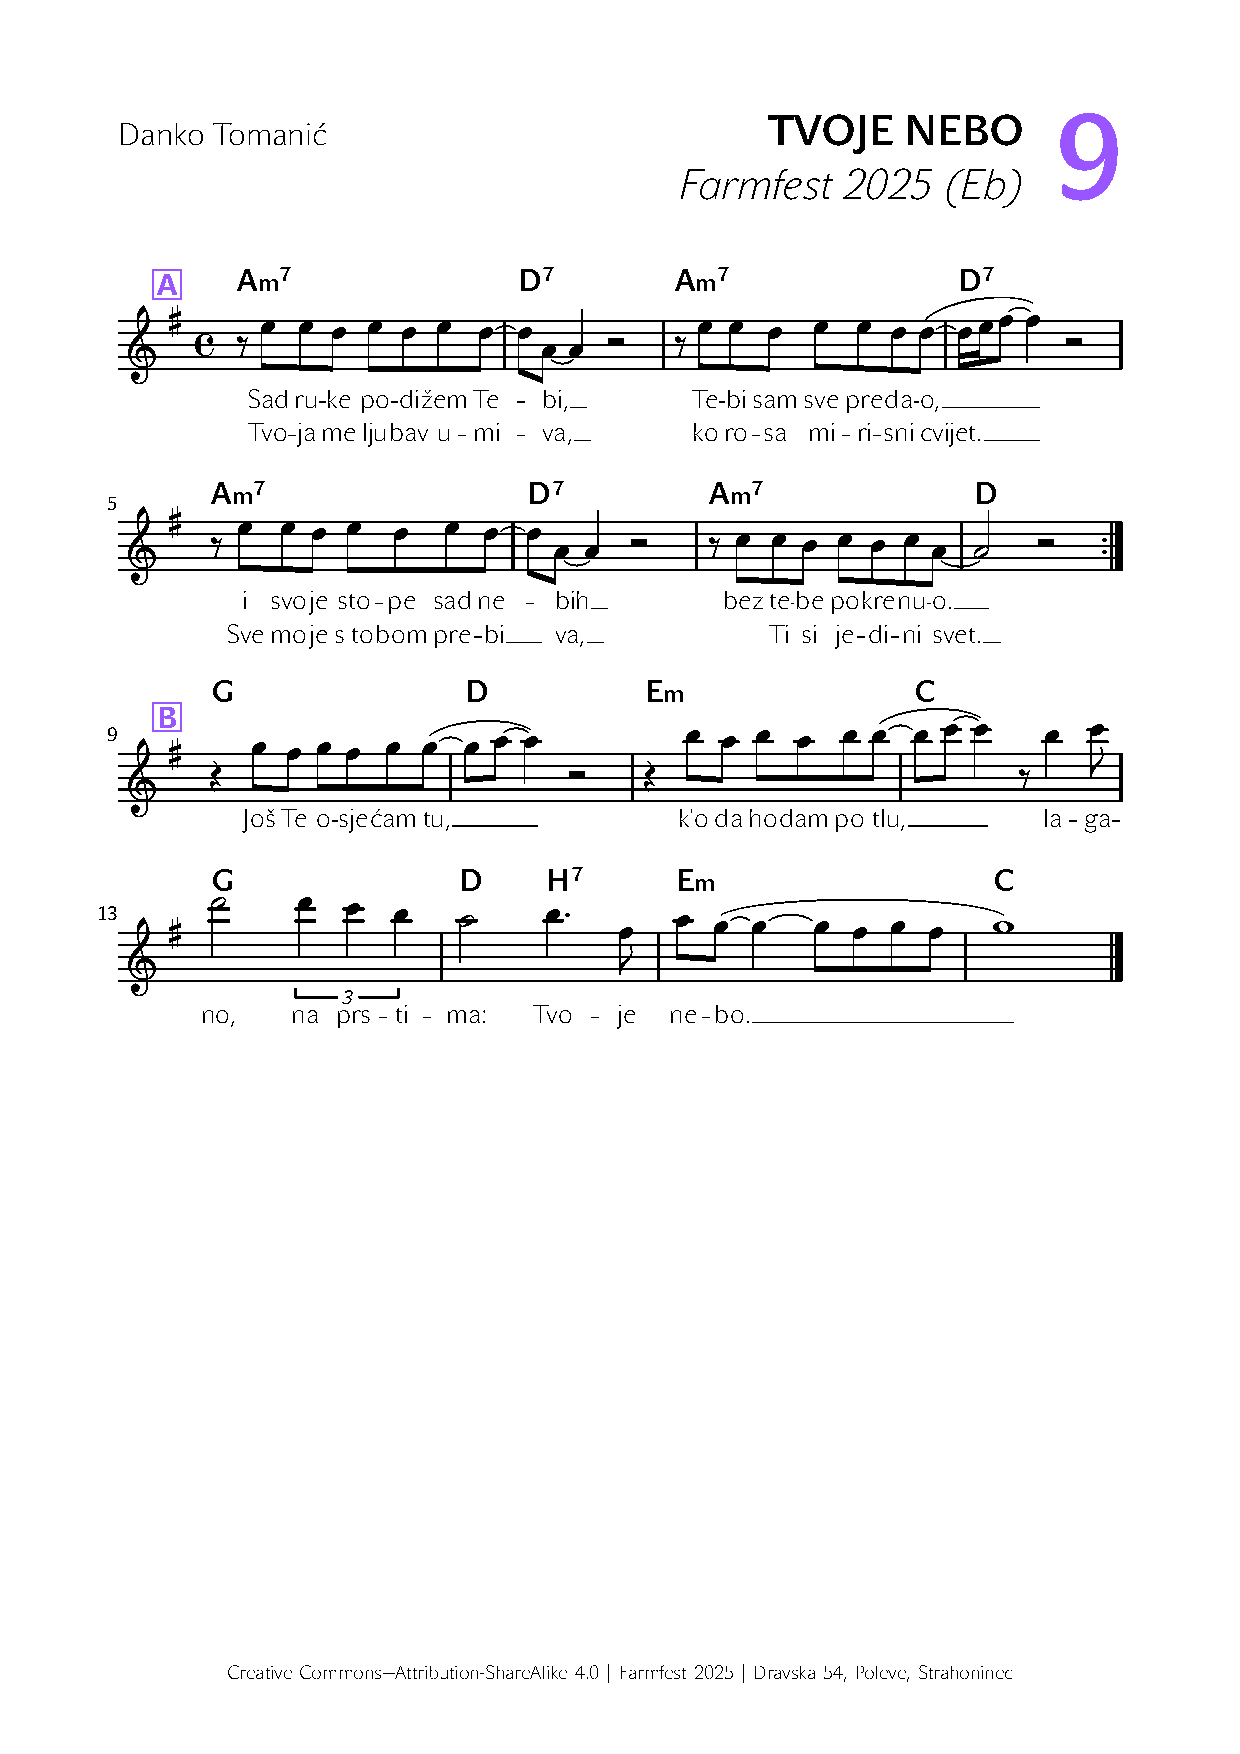
\includepdf[pages={1},noautoscale]{../lilypond/bin_eb/tvoje_nebo.pdf}
\end{minipage}

%pjesma 10
\newpage
\phantomsection
\begin{minipage}[b]{0.5\linewidth}
\addcontentsline{toc}{section}{\texorpdfstring{{\rednifont\doccolor10.}\hspace{\twodigitspacing}}{}U DUHU BUDITE GORLJIVI}
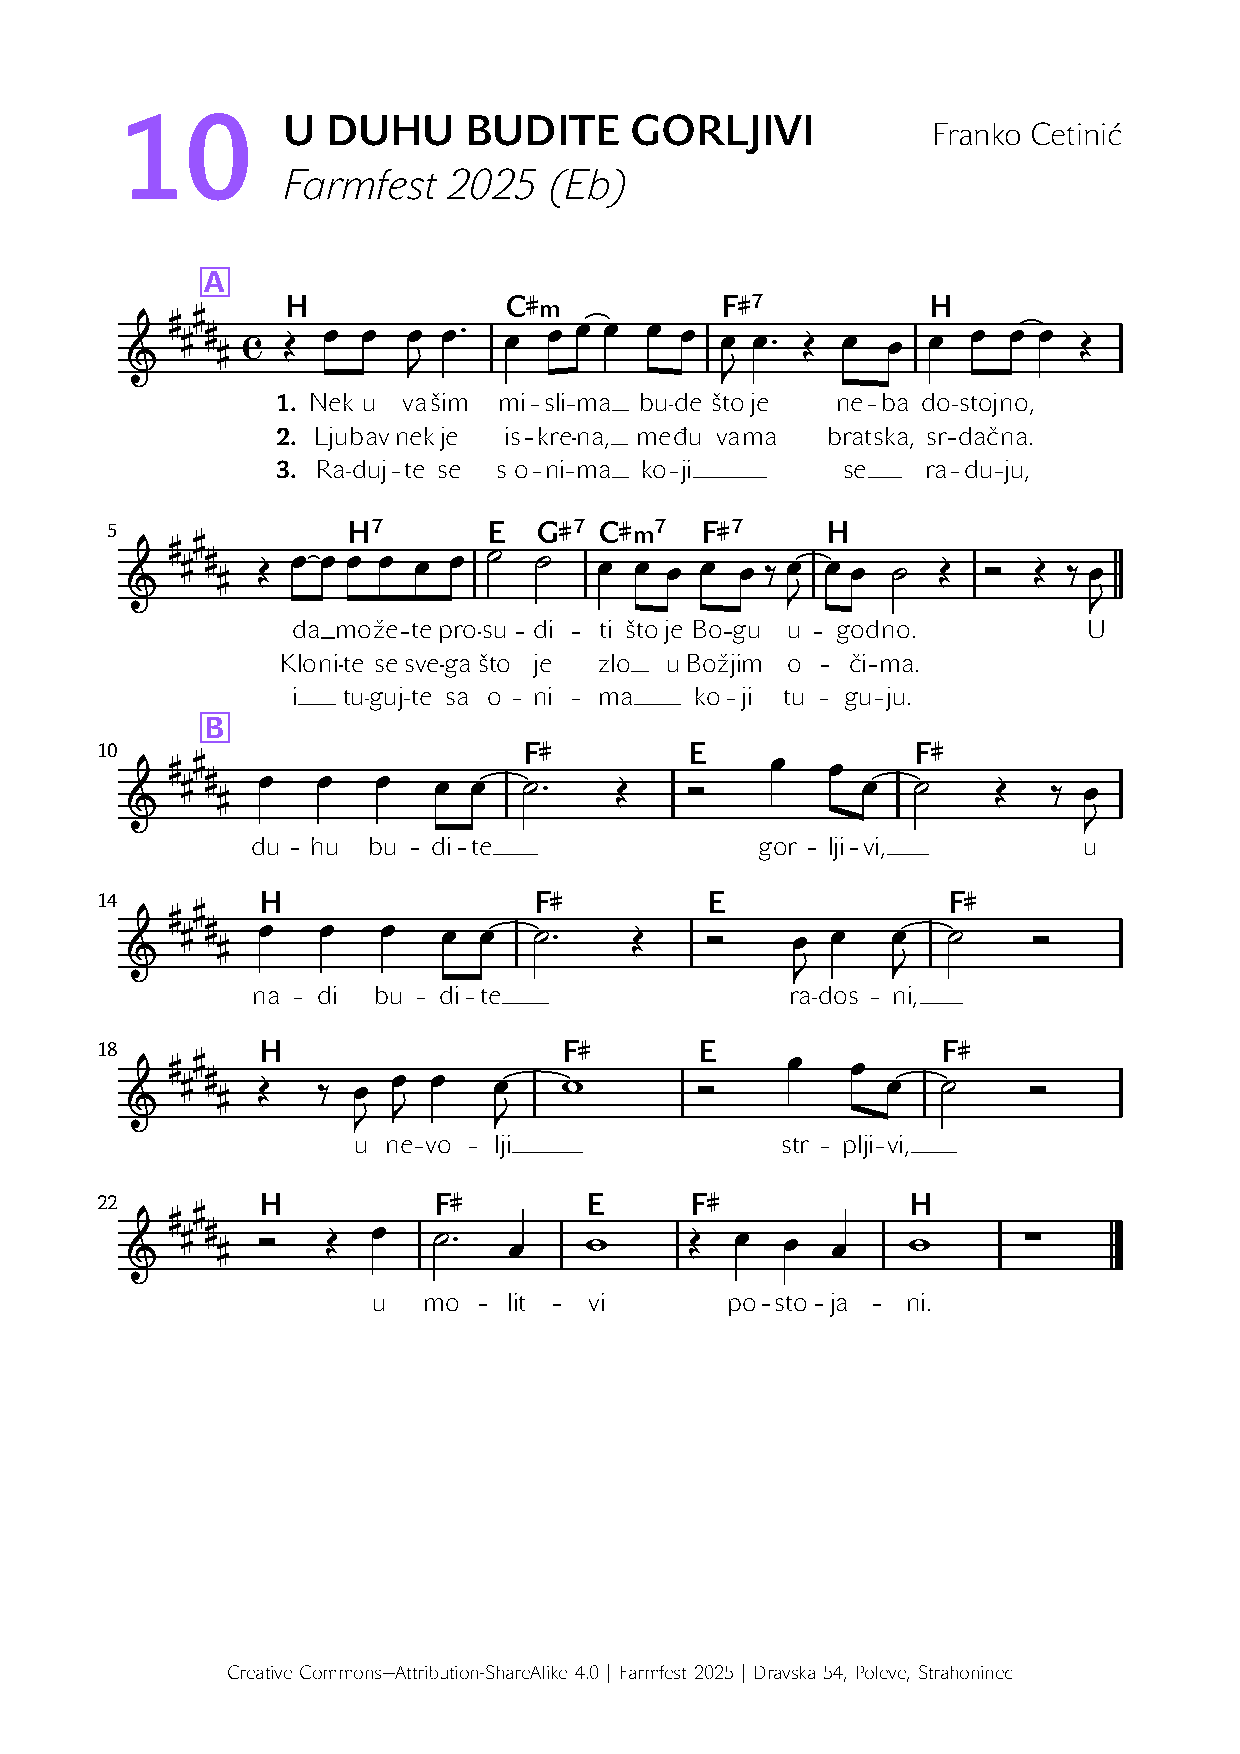
\includepdf[pages={1},noautoscale]{../lilypond/bin_eb/u_duhu_budite_gorljivi.pdf}
\end{minipage}

%slika
\newpage
%\vspace*{4cm}

\begin{center}
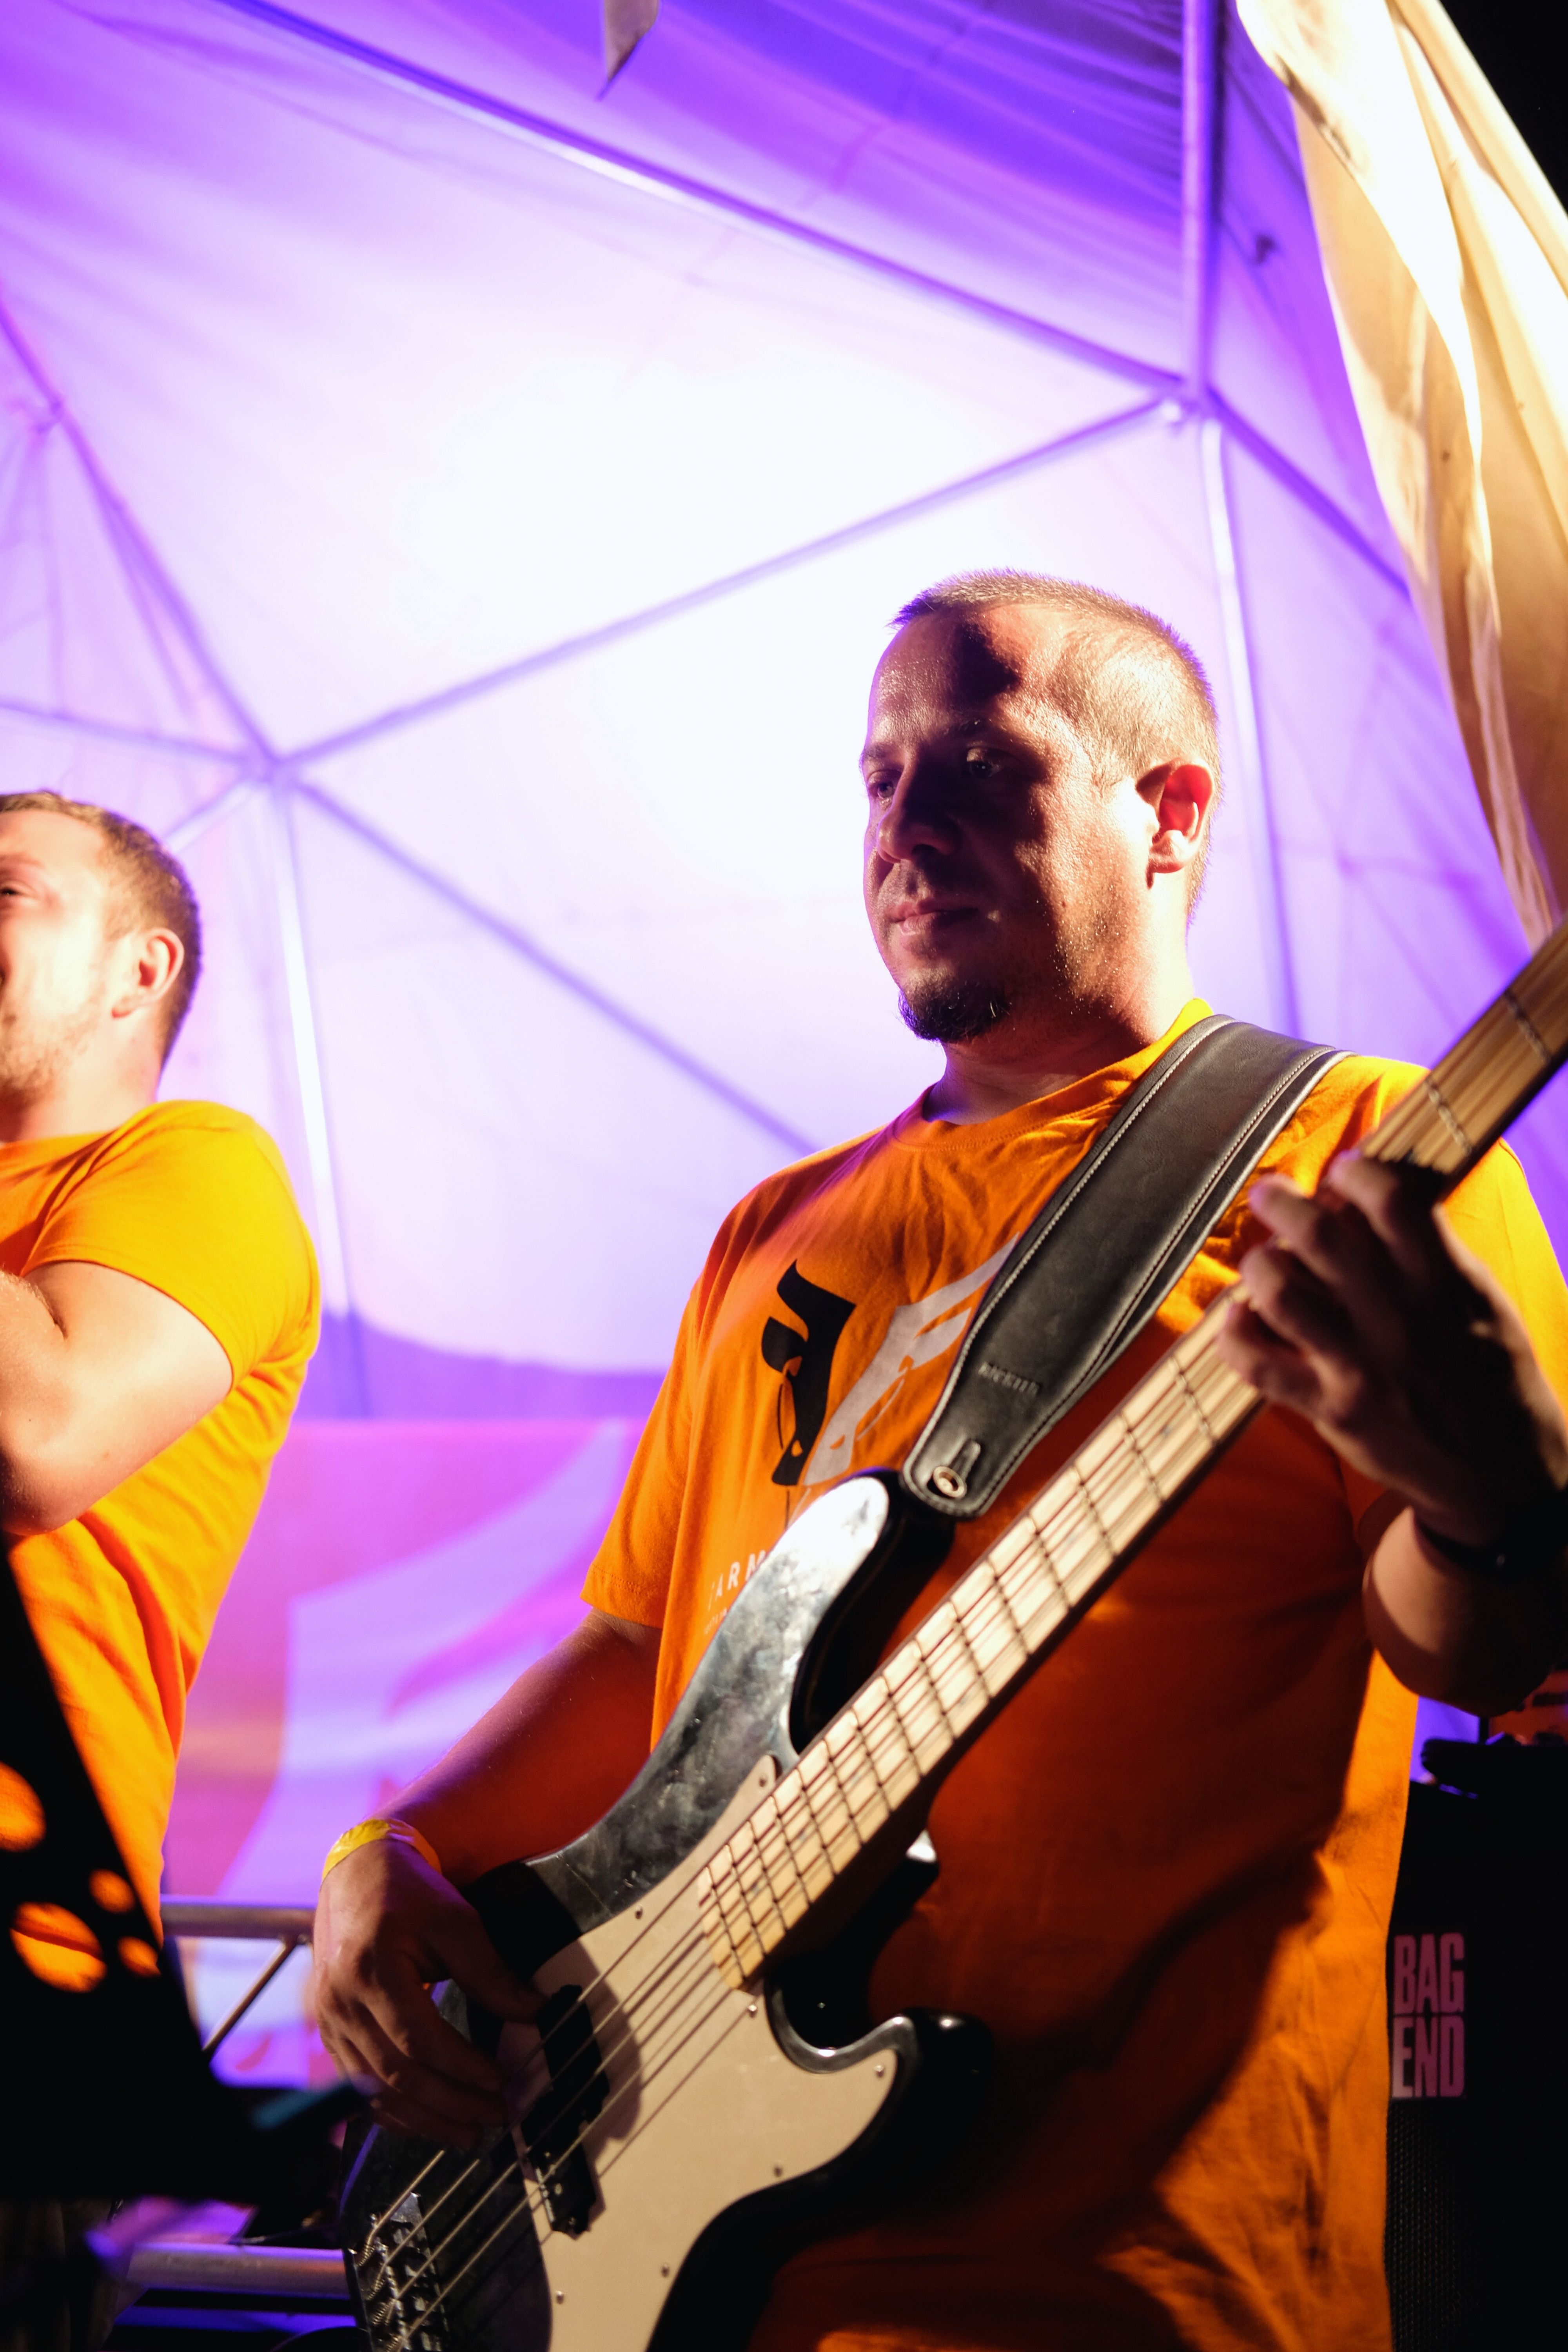
\includegraphics[width=400pt]{images/38.jpg}
\end{center}

\vspace*{1mm}
\begin{center}

	\Large{\parbox{\linewidth}{
		\begin{center}
		{\Large
		\texttt{
			\textit{"U Boga se uzdaj, jer opet ću ga slaviti,\\
spasenje svoje, Boga svog!"}
			}
		}
		\end{center}
		\begin{center}
		{\Large
			\texttt{{\textemdash Psalam 42,6}}
		}
		\end{center}
	}
}
\end{center}

%pjesma 11
\newpage
\phantomsection
\begin{minipage}[b]{0.5\linewidth}
\addcontentsline{toc}{section}{\texorpdfstring{{\rednifont\doccolor11.}\hspace{\twodigitspacing}}{}VIDJEH OBLAK}
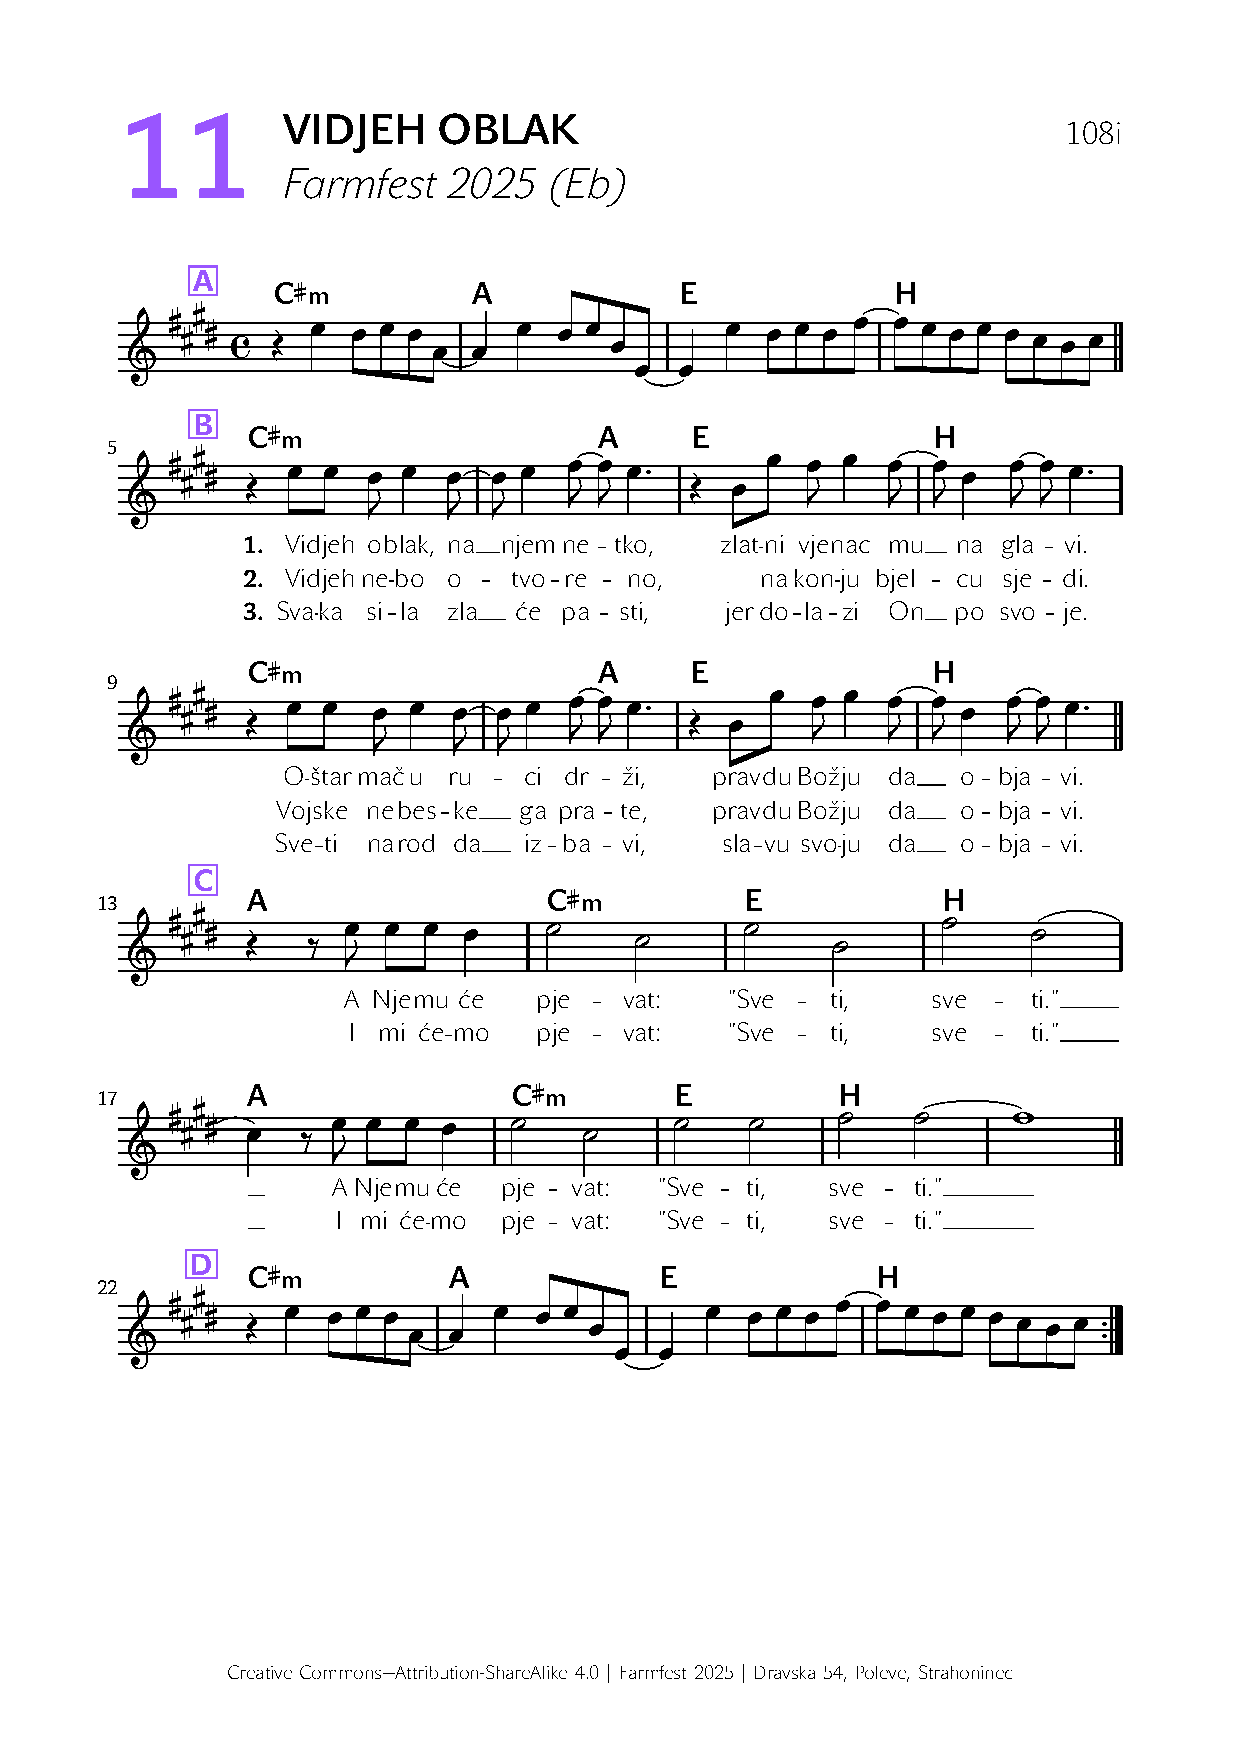
\includepdf[pages={1},noautoscale]{../lilypond/bin_eb/vidjeh_oblak.pdf}
\end{minipage}
\newpage
\includepdf[pages={2},noautoscale,
    picturecommand={\setlength\unitlength{1cm}%
         \put(2,6){\includegraphics[width=\linewidth]{images/8.jpg}}}]%
   {../lilypond/bin_eb/vidjeh_oblak.pdf}

\newpage
\notes[10pt]{29}{\textwidth}

\newpage
\pagenumbering{gobble}
\vspace*{10.7cm}
%\begin{center}
%    Inner side of back cover page. Remove!
%\end{center}
%\begin{center}
%    \textit{Unutarnja strana korica.}
%\end{center}

\newpage
\pagenumbering{gobble}
\includepdf[pages={1},noautoscale]{images/ff2026_korice_zadnja.pdf}

\end{document}
%#################################################################################
%   END OF DOCUMENT
%#################################################################################
